\part{Analyse acoustique du théâtre d'Orange}
\label{part3}

\chapter*{Introduction}
	\addcontentsline{toc}{chapter}{Introduction}
	
%\section{Interface utilisateur} \label{sect_add-on}
 Il est d'usage de prétendre que l'acoustique des théâtres antiques est excellente et que le son, par de simples astuces géométriques, est bien perçu à toutes les places. Mythe ou réalité ? On peut dans tous les cas constater que les romains adaptaient leurs architectures aux usages des bâtiments. Ainsi on pourra distinguer les théâtres antiques des \glspl{odeon} qui, plus petit et complètement fermés avaient un usage exclusivement musical. Les romains ainsi que les Grecs ont choisi de bâtir un type de bâtiment adapté aux représentations théâtrales et ont reproduit de manière assez similaire cette architecture globale en différents lieux. Quelles étaient donc les astuces architecturales permettant d'optimiser la propagation du son sachant que "les architectes [de l'antiquité] n'ont jamais disposé que de deux moyens : la géométrie et l'oreille" \cite[p.15]{canac} ? On sait par ailleurs que l'acoustique faisait parti des préoccupations des architectes puisque Vitruve, contemporain de l'époque Augustéenne en fait régulièrement état dans son \textit{De architectura} livre V. \cite[Livre V]{vitruve}. François Canac, a mené durant de nombreuses années une large étude théorique et expérimentale sur l'acoustique des théâtres antiques \cite{canac}. Il explique que l'excellente acoustique des théâtres antiques tel que celui d'Orange est dû à plusieurs facteurs géométriques :
\begin{itemize}
\item L'orchestre qui fonctionne comme un miroir et réfléchi le son provenant de la scène vers les gradins.
\item Le mur de scène qui réfléchi également le son vers les gradins. Pour que ce son réfléchi ne soit pas présent sous forme d'écho (ce qui nuirai grandement à la compréhensibilité) il est nécessaire que la scène soit peu profonde.
\item Les murs de scène s'élevaient presque toujours là où le terrain arrière était horizontal avec donc la possibilité de présenter des bruits parasites. Le mur semble donc avoir un rôle de "parason" \cite[p.38]{canac}.
\item L'angle des gradins qui augmente en générale lorsqu'on s'éloigne de la scène et qui permet à tous les spectateurs de bénéficier des réflexions sur l'orchestre \cite[p.103-109]{canac}.
\item Le caractère simple de la géométrie : des murs très réfléchissants des gradins à ciel ouvert permettant la presence de premières réflexions et peu de réverbération \cite[p.33]{canac}.
\item Le \gls{pulpitum} qui présente des niches alternativement rectangulaires et semi-circulaire (mais qui est plat dans les \glspl{odeon}) pourrait servir soit à disperser les échos nuisibles soit à faire résonner la musique \cite[p.38]{canac}.
\item Les gradins doivent permettre à l'acteur de s'entendre en retour afin d'avoir la sensation que sa voix porte \cite[p.42 - tab.II-4]{canac}.
\end{itemize}
L'un des caractère essentiel de l'étude acoustique dans un théâtre est la compréhensibilité. Nous ne disposons pourtant que de peu d'information dans ce domaine. Premièrement, il n'est pas impossible que certains spectacles de théâtre aient été non verbaux et plutôt de type pantomime. Par ailleurs, l'usage de la parole dans les représentations théâtrales est difficile à comprendre. Outre le fait que l'élocution était probablement très différente de celle qu'on connait aujourd'hui (Aristote \cite[Chap IV - XIV]{aristote} et Plutarque ont insisté sur l'entrainement rigoureux des acteurs pour développer leur voix et leur aisance sur scène \cite[p.39]{canac}) les acteurs portait probablement des masques amplificateurs pour amplifier leur voix \cite[p.362]{arnaud}. Il est rapporté par Philostrate dans \textit{La vie d'Apollonios de Tyane}, V, 9 "qu'un acteur tragique se rendit en occident et y fit une tournée ... Arrivé à Hyspalis (Seville) il sembla aux indigènes déjà effrayant par son aspect, bien qu'il n'eût pas encore prononcé une parole sur la scène. En le voyant marcher à grand pas, la bouche démesurément ouverte, monté sur des chaussures d'une hauteur extraordinaire, le corps dissimulé sous un étrange accoutrement, ces gens, n'étaient pas rassurés; mais quand il se mit à élever la voix et à déclamer sur un ton éclatant, la plupart prirent la fuite, comme poursuivis par les cris d'un démon". Il résulte donc de ce passage que la voix atteignait une sonorité considérable \cite[p.43]{formige}. C'est donc avec ces réserves que nous tenterons de comprendre comment la voix pouvait être transmise à l'aide de critères tels que la clarté \gls{C80} (voir section \ref{sect_data}).

Dans ce chapitre nous allons tenter d'aller plus loin dans l'analyse acoustique des théâtres antiques en utilisant des outils numériques. Effectivement, nous disposons désormais d'une maquette virtuelle du théâtre d'Orange ainsi que d'un outil de simulation acoustique, nous allons donc pouvoir combiner les deux pour tester différentes hypothèses archéologiques. Quel était l'impact de la position des spectateurs dans les gradins ? Le toit ou le \gls{velum} avaient-ils une incidence sur le son perçu ? Quels rôles jouent et jouaient les différents matériaux ? Voici quelques exemples auxquels nous tenterons d'apporter des réponses. Cette troisième partie commence par la présentation de la configuration initiale de la maquette virtuelle du théâtre d'Orange et de son analyse. Des calculs seront ensuite effectués pour différentes configurations du théâtre afin de les comparer aux résultats de référence et ainsi d'éclairer certaines hypothèses de reconstitution. Nous verrons finalement dans un contexte plus général comment se situe le théâtre d'Orange par rapport à d'autres théâtres en terme d'acoustique.	
	

	
\chapter{Analyse en configuration initiale}
	\citationChap{
	Les idées sont comme des êtres vivants. Elles naissent, elles croissent, elles prolifèrent, elles sont confrontées à d'autres idées et elles finissent par mourir.
	}{Bernard Werber}
	\minitoc
	\newpage
	

	\section{Configuration du maillage}
Pour effectuer les tests nous mettons en place une configuration de référence. Celle-ci sera détaillée et étudiée dans ce chapitre tandis que le chapitre suivant présentera l'impact des différents éléments sur l'acoustique du bâtiment. Nous pourrons alors procéder de manière relative en ôtant les éléments les uns après les autres pour constater leur impact. Cette configuration de référence est un parti pris de ce que nous pensons être le théâtre dans un état d'usage standard de représentation, c'est-à-dire restitué de manière quasi-complète, avec du public et sans \gls{velum}. Il est important de noter que cette configuration intègre des éléments hypothétiques (tel que de toit de la scène par exemple) mais dont l'aspect et la présence sont probables d'après ce que nous avons vu dans la partie \ref{part_1}. Cette configuration de référence est donc composée : du mur de scène et d'une partie de sa décoration (les colonnes, les \glspl{podium} et les entablements), de l'\gls{orchestra}, de la scène et de sa couverture, des basiliques, des \glspl{aditus} et de la \gls{cavea} ainsi que de la \gls{porticus isc} (voir fig. \ref{theatreMat}). On ajoute également les trois grandes portes du \gls{postscaenium} ainsi que les diverses niches qui ont été modélisées sur le front de scène (voir Chap. \ref{mur}). Ce sont les éléments qui peuvent avoir un impact non négligeable sur l'étude acoustique. Nous pouvons noter que le maillage ainsi constitué comporte environ 160~000 triangles. Notons également que le décor du front de scène est légèrement déraffiner grâce au \gls{decimate} afin d'alléger le maillage. Les tests acoustique auront tous lieu à l'intérieur du bâtiment, ainsi, certains éléments situés à l'extérieur de l'enceinte ont été ôtés du model tels que les arcades autour de la \gls{cavea}, les mâts de \gls{velum}, etc. 

En ce qui concerne les matériaux, nous avons tenté de se rapprocher de la réalité d'après les éléments disponibles aujourd'hui. Tous les éléments construits en grand appareil sont en calcaire de Courthezon \cite[p.43]{orangeTxt}. L'orchestre était à priori dallé avec un matériau de type marbre \cite[p.337]{orangeTxt}. On utilisera également du marbre pour le front du \gls{pulpitum}, le décor du front de scène et la \gls{porticus isc}. Le front de scène, derrière sa décoration était orné de panneaux mêlant probablement du marbre varié et polychrome ainsi que des mosaïques, nous lui assignerons donc également un matériau de type marbre. Le plancher de la scène, les portes du \gls{postscaenium} ainsi que les couvertures de la scène et de la \gls{porticus isc} étaient à priori en bois (probablement du chêne pour ses propriétés mécaniques et sa présence régionale). Notons que seules les faces donnant vers l'intérieur du théâtre nous importent, c'est pourquoi nous ne traiterons pas des matériaux recouvrant les toitures. Enfin, la configuration initiale se fait avec le public puisque c'est le cas d'utilisation le plus courant. Nous assignons donc aux gradins un matériau de type audience tout comme aux trois degrés bas situés sur l'orchestre et réservés au Sénateurs. Dans la base de donnée d'Odéon \cite[materials]{odeon} on récupére les matériaux qui se rapprochent le plus de ceux évoqués précédemment et on obtient les coefficients d'absorption correspondant (voir tab. \ref{matOdeon}). Ce qui saute aux yeux dans ce tableau c'est que le calcaire et le marbre sont extrêmement réfléchissant et semblent tenir une fonction de miroir acoustique. A contrario le public est plutôt absorbant et on imagine que son rôle sera de limiter les échos. Quant au bois, il absorbe moyennement les basses fréquences et peu les hautes fréquences. Notons également que nous assignons aux ambulacres un matériau 100\% absorbant afin d'éviter que des rayons ne se perdent dans les couloirs sans en ressortir, ce qui rallongerait le temps de calcul.
%
\begin{tableth} 
\footnotesize
	\begin{tabular}{| m{1.5cm} | c | m{1.7cm} | *{8}{c|}}
		\hline
		Matériau &Réf & Equivalent Odéon & 62,5Hz & 125Hz & 250Hz & 500Hz & 1kHz & 2kHz & 4kHz & 8kHz \\
		  \hline
		  \hline
		   Calcaire & 1001 & Smooth brickwork with flush pointing\footnotemark & 0.02&	0.02&	0.03&	0.03&	0.04&	0.05&	0.07&	0.07 \\
		   \hline
		Marbre &2001 & Marble or glazed tile\footnotemark & 0.1 & 0.1 & 0.1 & 0.1 & 0.1 & 0.2 & 0.2 & 0.2 \\
		   \hline
		Bois & 3000 & Hollow wooden podium\footnotemark & 0.4&0.4&0.3&	0.2&	0.17& 0.15& 0.1&	0.1 \\
		   \hline
		Public sur gradins & 11009 & Audience, lightly upholstered seats\footnotemark & 0.51&	0.51&	0.64&	0.75&	0.8&0	0.82&	0.83&	0.83 \\
	     \hline
	     	Public sur sièges mobiles & 11003 & Audience on wooden chairs, 1per sq.m\footnotemark & 0.16 & 0.16 & 0.24 & 0.56 & 0.69 & 0.81 & 0.78 & 0.78 \\
	     \hline

	 \end{tabular}
	\caption{Matériaux et les coefficients d'absorption correspondant du théâtre d'Orange}
	\label{matOdeon}
\end{tableth}
\addtocounter{footnote}{-1}
\footnotetext{Bobran, 1973}
\addtocounter{footnote}{-1}
\footnotetext{Harris, 1991}
\addtocounter{footnote}{-1}
\footnotetext{Dalenbäck, CATT}
\addtocounter{footnote}{1}
\footnotetext{Beranek, Hidaka, 1998}
\addtocounter{footnote}{1}
\footnotetext{Meyer, Kunstmann, Kuttruff, 1964}

\begin{figureth}
	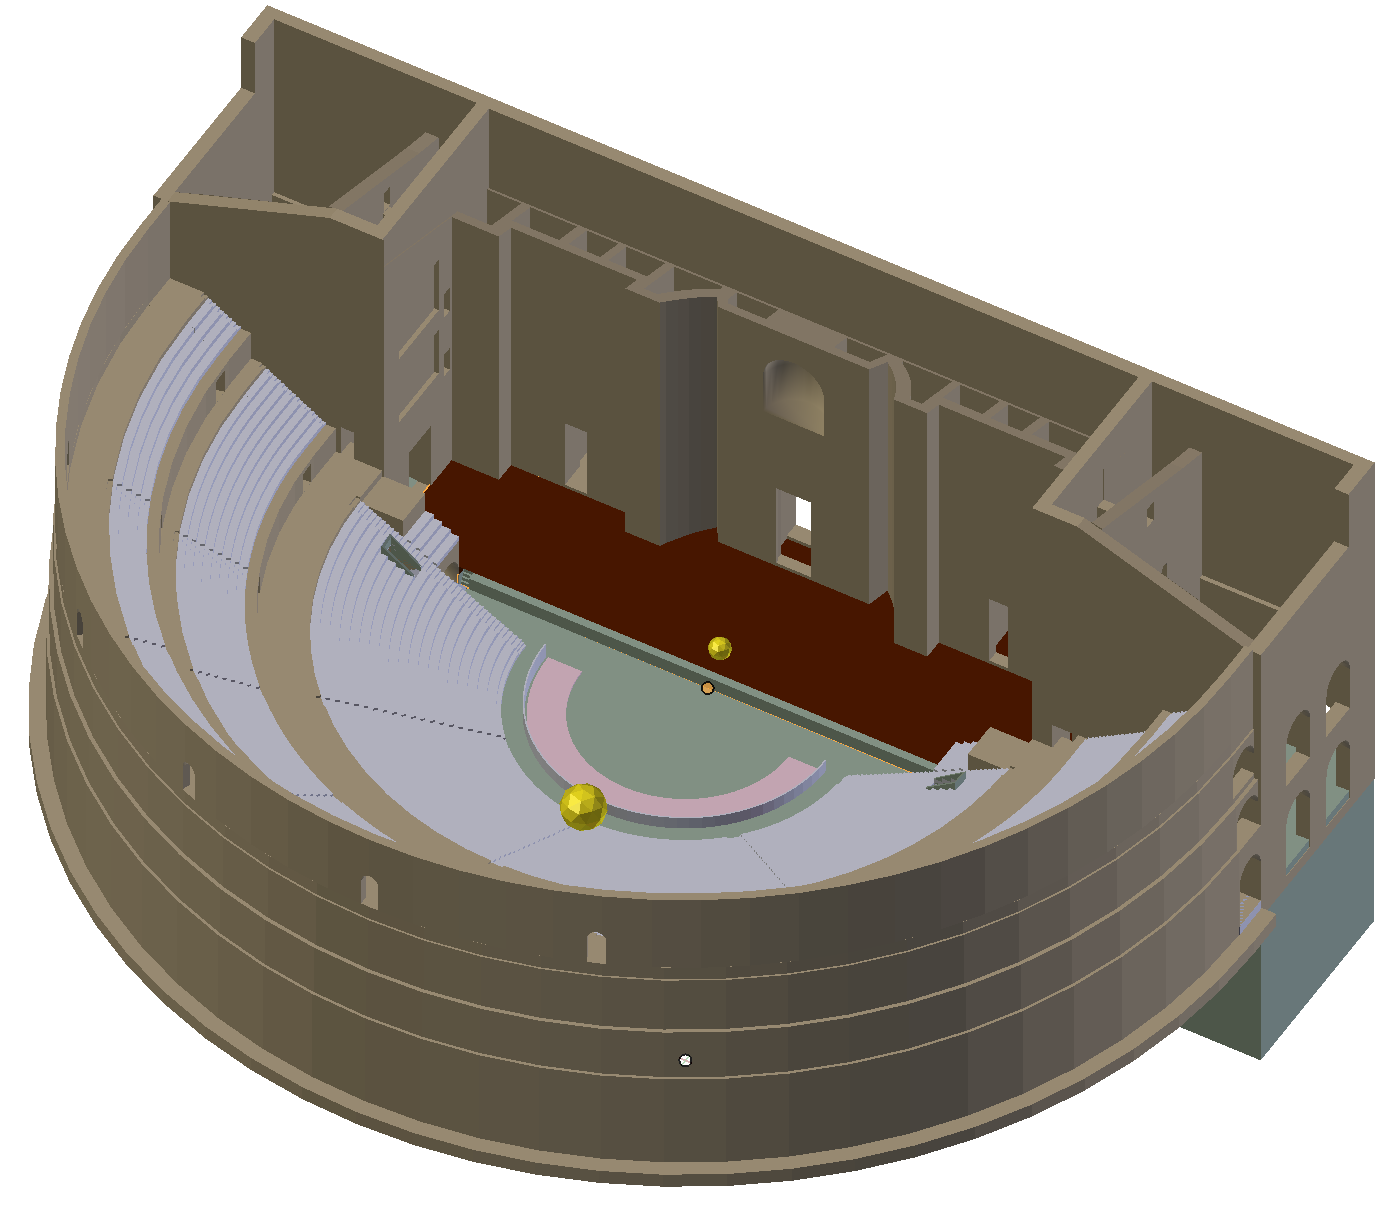
\includegraphics[width=\linewidth]{images/theatreMat}
	\caption{Représentation des matériaux sur le théâtre d'Orange : Calcaire (beige), Marbre (vert), Bois (orange), Audience sur gradins (gris), Audience sur siège en bois (rose) ainsi que la source (rouge) et le récepteur (jaune) dans la configuration initiale.}
	\label{theatreMat}
\end{figureth}

On peut voir sur la figure \ref{theatreMat} la répartition des différents matériaux sur sur le bâtiment. Nous plaçons une source sonore centrée sur la largeur de la scène à 160cm au dessus de celle-ci (environ la hauteur d'une bouche humaine) soit à une altitude de 42,8m et à 2m du bord. Nous choisissons cette position comme position de source initiale. Le récepteur initial est situé dans le même axe, c'est-à-dire au centre des gradins et à la même altitude. Sa distance par rapport au centre de l'orchestre est de 16,5m, ce qui correspond aux gradins 3 à 8 environ. Son rayon de mesure sera de 2m. 

Nous testons le calcul complet avec un et deux millions de rayons. Nous constatons que les résultats sont quasiment identiques à partir de 500Hz mais que les temps de réverbération sont un peu plus grand pour les basses fréquences à deux millions de rayons (moins de 10\% d'écart). Cela s'explique par le fait que l'atmosphère ainsi que les matériaux atténuent très peu ces fréquences. Cependant, ce faible écart de résultats reste acceptable compte tenu de la diminution du temps de calcul. Il est de 50min pour deux millions de rayons et 20min pour un million. Nous testons aussi le calcul pour 500~000 rayons dont le temps est de 7min et retrouvons des résultats identiques à la configuration à deux millions de rayons au delà de 4kHz. Pour les plus basses fréquences l'écart va jusqu'à 17\%. Nous choisissons donc de travailler avec un million de rayons.



\section{Analyse de la réponse impulsionnelle}

%L'analyse de l'acoustique d'une salle peut se faire à l'aide de différents facteurs perceptifs tel que le \gls{RT60} que nous avons décrit précédemment. 
%La \gls{rir} de la configuration décrite précédemment pour un \gls{RT60} est présentée figure \ref{rirTheatre}.

\begin{figureth}
	\begin{subfigureth}{\linewidth}
		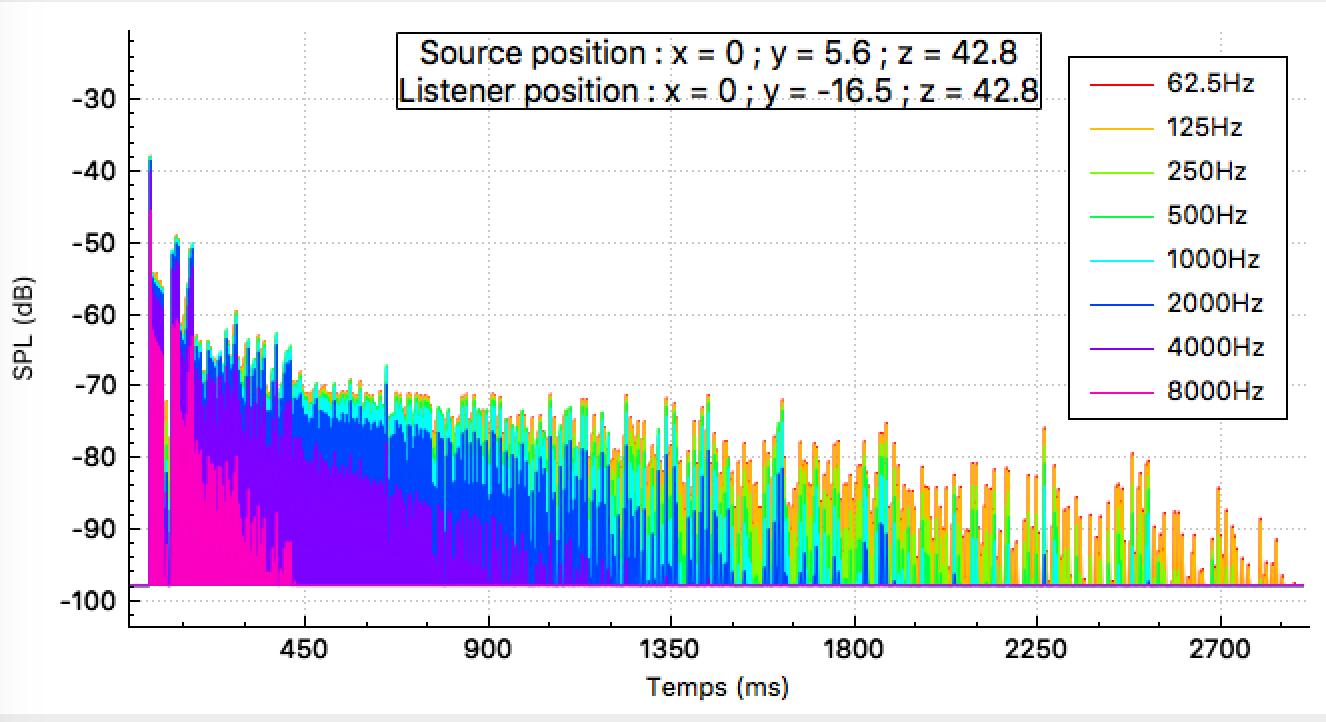
\includegraphics[width=\linewidth]{images/rirTheatreAvecDecor}
			\caption{Réponse impulsionnelle jusqu'à -60dB.}
		\label{rirTheatre60}
	\end{subfigureth}
	\begin{subfigureth}{\linewidth}
		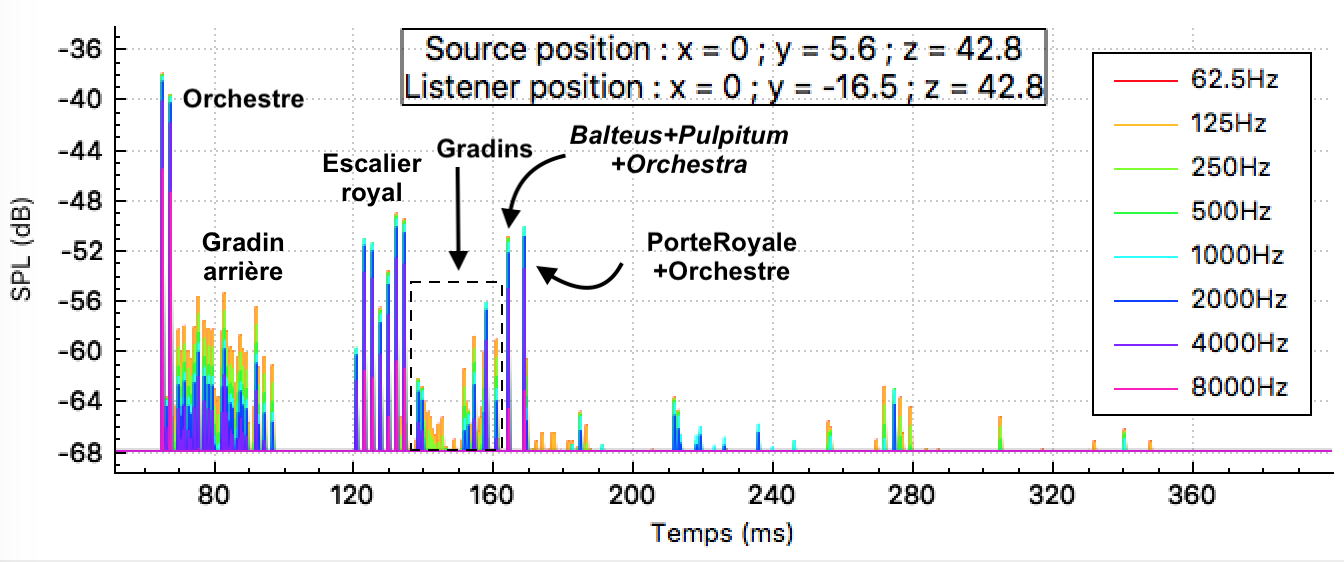
\includegraphics[width=\linewidth]{images/rirTheatre30bis}
		\caption{Réponse impulsionnelle jusqu'à -30dB.}
		\label{rirTheatre30}
	\end{subfigureth}
		\begin{subfigureth}{\linewidth}
		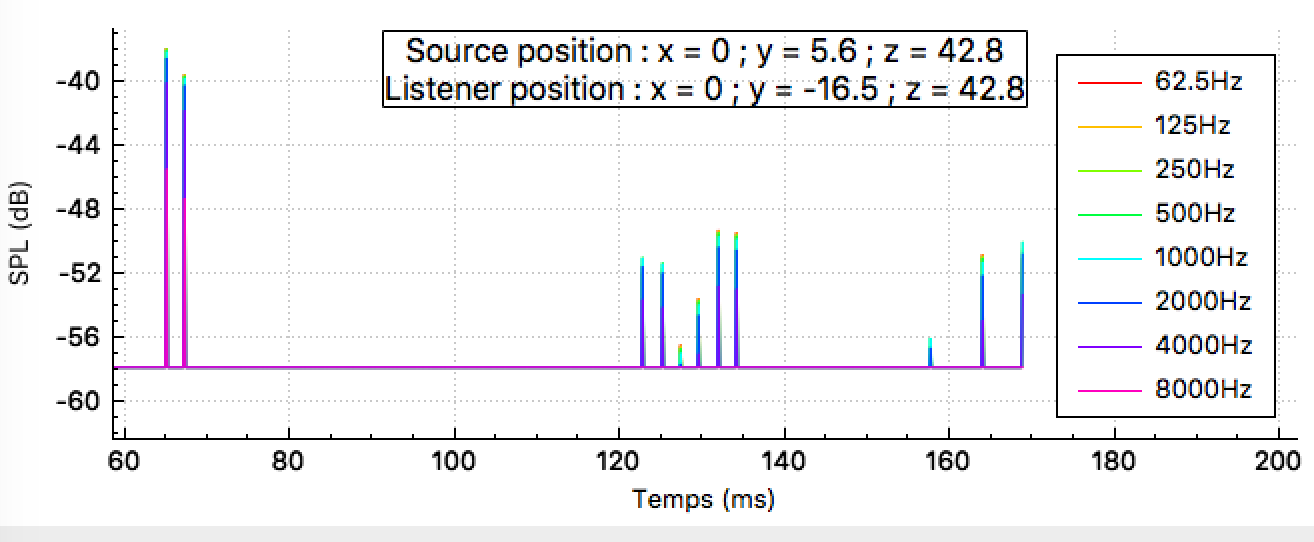
\includegraphics[width=\linewidth]{images/rirTheatre20}
		\caption{Réponse impulsionnelle jusqu'à -20dB.}
		\label{rirTheatre20}
	\end{subfigureth}
	\caption{\gls{rir} du théâtre d'Orange dans sa configuration initiale pour 1 million de rayons.}
	\label{rirTheatre}
\end{figureth}

La figure \ref{rirTheatre} et le tableau \ref{tab_fact_init} illustrent les caractéristiques de  la réponse impulsionnelle de la configuration initiale. On constate un \gls{RT60} de l'ordre de 3 secondes environ. Grâce aux figures \ref{rirTheatre30} et \ref{rirTheatre20} nous allons pouvoir analyser d'où proviennent les pics d'énergies les plus forts. Pour cela, nous nous appuyons sur les travaux de Haas et Meyer \cite[p.49]{haas} qui expliquent à quel moment une réflexion devient un écho :
\begin{itemize}
\item si l'intervalle entre le son direct et le son réfléchi est inférieur à 5ms, l'auditeur entend un son unique dont l'intensité est la somme des deux signaux. La direction perçue est la bissectrice de l'angle formé par les deux sources (réelle et virtuelle) ;
\item si le temps entre les deux signaux est compris ente 5 et 35ms, l'intensité est encore la somme des intensités mais la direction est celle du premier signal ;
\item si le temps entre les deux signaux est compris entre 35 et 50ms, les deux signaux sont distingués dans le temps mais la direction semble être celle du premier son ;
\item au delà de 50ms, les deux signaux sont complètement distingués dans le tmps et l'espace.
\end{itemize}
Sur la figure \ref{rirTheatre20} on constate la présence d'un pic de signal 5ms après le son direct ce qui entre dans le premier cas décrit précédemment. Après analyse, nous constatons que celui-ci provient de la réflexion sur l'orchestre. L'orchestre va donc doubler l'intensité sonore émise depuis l'avant scène. Sur la figure \ref{rirTheatre30} nous constatons qu'il y a ensuite beaucoup de signal dispersé sur environ 30ms qui correspond aux rayons réfléchis sur le dossier des gradins et qui reviennent converger sur le récepteur (voir fig \ref{SI30dB}). Une partie d'entre eux se sont également réfléchis sur l'orchestre ajoutant encore à l'impact de cette surface dallée. D'après les critères de Haas évoqués précédemment, ces signaux sont parfaitement confondus avec le son direct. Il y a ensuite un trou de 20ms avant les prochains pics. Ceux-ci étant retardés de plus de 50ms par rapport au son direct, ils pourront être perçus comme un écho. Ces derniers proviennent des réflexions sur les marches d'escalier de la porte royale. Il est bon de rappeler que nous utilisons une source omnidirectionnelle et qui, à la différence de la voix humaine envoie autant d'énergie vers le mur que vers les gradins. Par ailleurs, nous sommes dans l'approximation hautes fréquences où l'on néglige certains effet de diffraction. On peut donc s'attendre à avoir un signal un peu différent dans la réalité même si notre étude permet de se faire une bonne idée du comportement acoustique du bâtiment. À 160ms les quelques pics présents sont dûs aux rayons réfléchis sur les gradins qui, bien que fortement atténués par le matériau arrivent en phase et jouent donc un rôle non négligeable dans la réverbération. Il y a ensuite deux grands pics à -10dB issus de multiples réflexions. Le premier est dû aux réflexions successives sur le \gls{balteus}, le font du \gls{pulpitum} et l'orchestre. Le deuxième provient de réflexions au niveau de la porte royale et de l'orchestre. L'agencement de ces deux parties (le \gls{balteus} et la porte royale) étant très hypothétiques, il faudra considérer la présence de ces deux pics comme peu fiable.
%
\begin{figureth}
	\begin{subfigureth}{0.8\textwidth}
		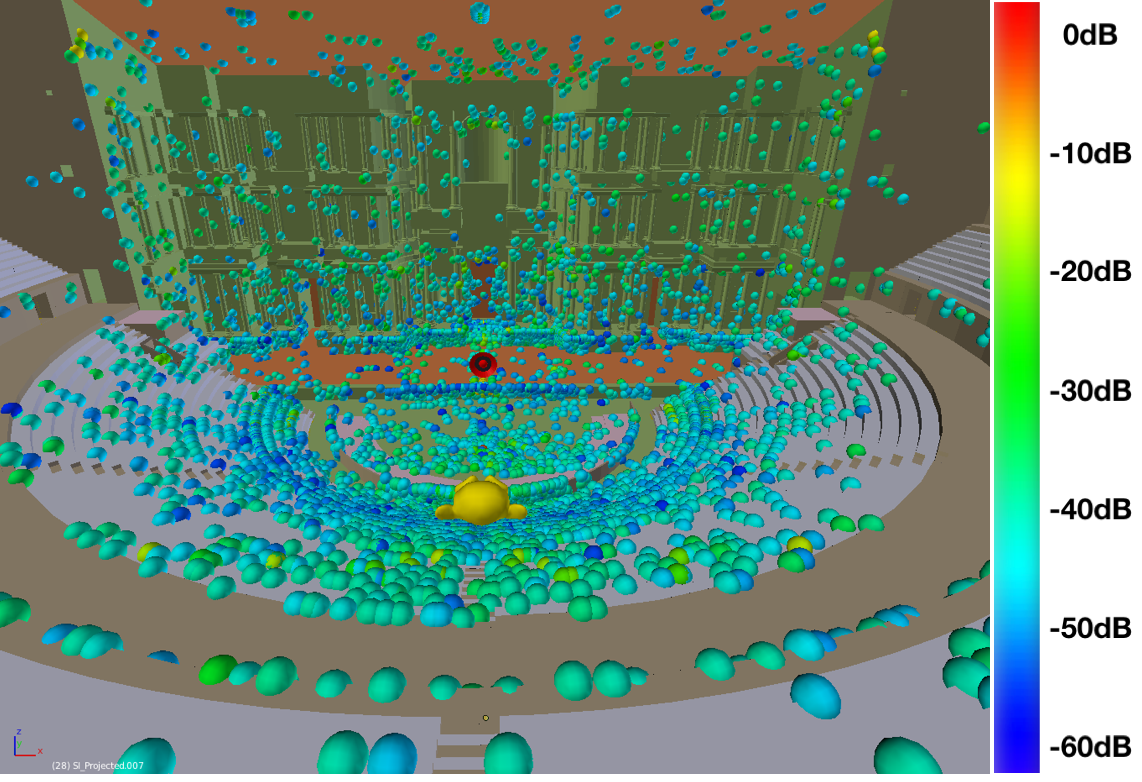
\includegraphics[width=\linewidth]{images/SI60dB}
		\caption{Source-images projetées sur les parois du théâtre jusqu'à -60dB vu des gradins.}
		\label{SI60dB}
		\hfill
		\quad
	\end{subfigureth}
	
	\begin{subfigureth}{0.8\textwidth}
		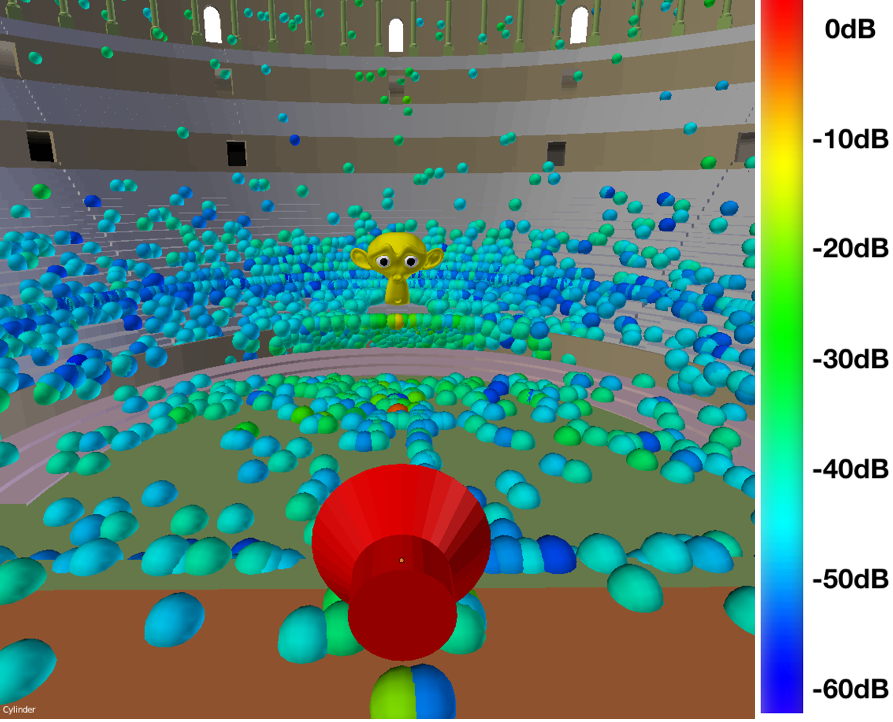
\includegraphics[width=\linewidth]{images/SI60dBbis}
		\caption{Source-images projetées sur les parois du théâtre jusqu'à -60dB vu de la scène.}
		\label{SI60dBbis}
		\quad
	\end{subfigureth} 
\caption{Source-images dans le théâtre d'Orange dans sa configuration initiale pour 1 million de rayons.}	
\label{SITheatre60}
\end{figureth}
%
En ce qui concerne la position des sources-images on constate clairement que pour une mesure à -60dB il y a des sources-images tout autour du récepteur avec de fortes concentrations sur les premiers gradins, sur l'orchestre, sur la scène et sur le bas du mur (voir fig. \ref{SI60dB}). C'est finalement à proximité du plan source-récepteur que se concentre la majeur partie des sources-images. Cependant on constate la présence de sources-images au niveau de la niche centrale et des différentes \glspl{precinction} ce qui implique que le son qui monte peut aussi redescendre vers les gradins du bas (voir fig. \ref{SI60dBbis}). En observant les sources-images dont le niveau est supérieur à -30dB par rapport au son direct (voir fig. \ref{SITheatre30}), on peut confirmer la provenance des pics d'énergie de la figure \ref{rirTheatre30} décrite précédemment. 

La tableau \ref{tab_fact_init} présente les facteurs perceptifs de cette configuration initiale. Ces données confirment un temps de réverbération de l'ordre de 3s. Il est interessant de constater que ce temps est supérieur du temps de réverbération optimal pour la parole décrit par J.Jouhaneau \cite[p.209]{jouhaneau} et qui se trouve être légèrement inférieur à 2s. Ce dernier est obtenu à partir des courbes de pourcentage d'intelligibilité et de niveau sonore qui se croisent en ce point optimal. Effectivement, la réverbération d'une salle permet d'amplifier le niveau sonore de la voix, donc d'être mieux entendue mais, lorsque le signal se diffuse plus longtemps, il devient plus difficile de dissocier et comprendre les mots. Ce temps optimal est empirique et discutable puisque J.Jouhaneau décrit lui-même les limites de cette analyse dépendant du volume et du signal émis \cite[p.218]{jouhaneau}. Ce manque de compréhensibilité est corroboré par l'analyse des autres facteurs. Tout d'abord, on constate que la définition \gls{D50} et la clarté \gls{C80} augmentent avec la fréquence. Nous savons que les hommes lorsqu'ils utilisent une voix de poitrine émettent des fréquences de 80 à 400Hz environ tandis que les femmes, en voix de têtes, émettent des fréquences de 300 à 1500Hz \cite[Mécanismes vocaux]{voix}. Cependant, seuls les hommes étaient acteurs de théâtre à l'époque impériale. On en conclue que la compréhensibilté de leur voix n'était pas excellente mais plutôt moyenne. Elle serait plutôt adaptée à la musique puisqu'on dit que dans ce cas la clarté doit se situer entre -3dB et +3dB \cite[p.59]{acoustique}. Le temps central \gls{Ts} étant supérieur à 50ms et l'\gls{EDT} étant supérieur à 1s, on comprend d'autant plus que le signal va s'étaler et que les syllabes seront peu distinctes. En ce qui concerne le niveau sonore, on constate que le théâtre présente un gain compris entre 3 et 6dB selon la fréquence. Cela signifie que le bâtiment a un effet bénéfique pour la transmission du son puisqu'il double le niveau sonore des plus hautes fréquences et quadruple celui des basses fréquences. On retrouve bien l'analyse faite précédemment sur l'orchestre qui double le niveau sonore de la source. Le \gls{LF80} nous indique quant à lui une sensation d'éloignement par rapport à la source ce qui n'est pas étonnant au vu des dimensions du théâtre.

C'est donc à partir de cette analyse initiale que nous allons pouvoir comparer différentes configurations du bâtiment et en déterminer l'impact sur l'acoustique.
% 
\begin{figureth}	
	\begin{subfigureth}{0.36\textwidth}
		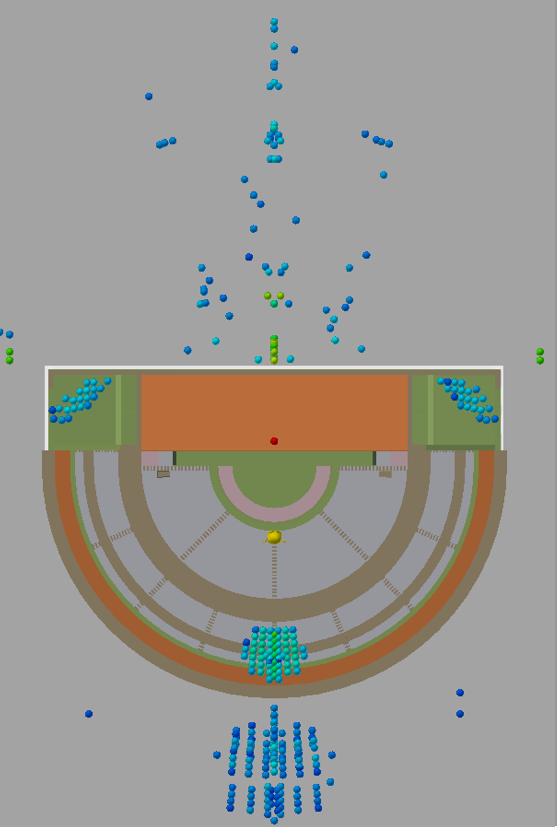
\includegraphics[width=\linewidth]{images/SI30dBbis}
		\caption{Source-images spatialisées jusqu'à -30dB.}
		\label{SI30dBbis}
	\end{subfigureth}
	\begin{subfigureth}{0.61\textwidth}
		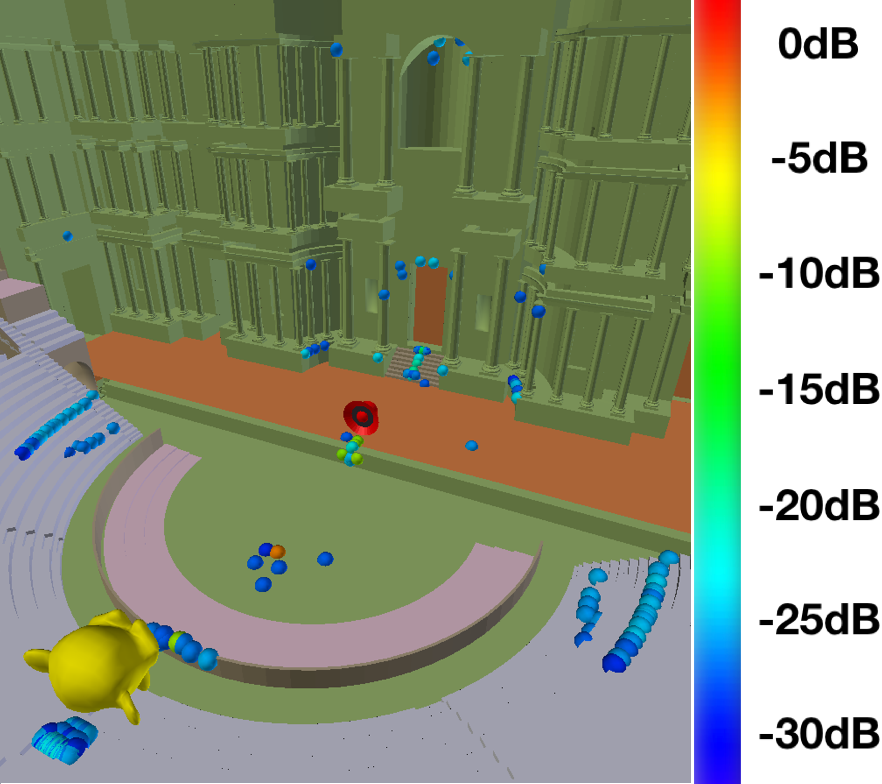
\includegraphics[width=\linewidth]{images/SI30dB}
		\caption{Source-images projetées sur les parois du théâtre jusqu'à -30dB.}
		\label{SI30dB}
	\end{subfigureth}
\caption{Source-images dans le théâtre d'Orange dans sa configuration initiale pour 1 million de rayons.}	
\label{SITheatre30}
\end{figureth}


\begin{tableth}
 \begin{tabular}{| *{9}{c|}} 
 \hline 
 Facteur & 62,5Hz & 125Hz & 250Hz & 500Hz & 1kHz & 2kHz & 4kHz & 8kHz \\ 
 \hline 
 \hline 
\gls{EDT} (ms)& 1867& 1854& 1636& 1501& 1323& 1130& 623& 387 \\ 
 \hline 
\gls{T30} (ms)& 3417& 3416& 3211& 2966& 2700& 2218& 1383& 672 \\ 
 \hline 
\gls{RT60} (ms)& 3155& 3130& 2822& 2606& 2420& 2057& 1425& 618 \\ 
 \hline 
\gls{spl} (dB)& -32& -32& -32& -32& -33& -34& -36& -42 \\ 
 \hline 
\gls{G} (dB)& 6.4& 6.4& 5.9& 5.5& 5.3& 5& 4.4& 3.5 \\ 
 \hline 
\gls{C80} (dB)& 2.4& 2.43& 3.14& 3.65& 4.1& 4.99& 7.01& 12.22 \\ 
 \hline 
\gls{D50} (\%)& 53.78& 53.96& 56.75& 58.48& 60.3& 64.04& 72.12& 86.9 \\ 
 \hline 
\gls{Ts} (ms)& 106& 105& 89& 81& 73& 59& 37& 14 \\ 
 \hline 
\gls{LF80} (dB)& 0.003& 0.003& 0.003& 0.002& 0.002& 0.002& 0.001& 0.001 \\ 
 \hline 
\end{tabular} 
 \caption{Facteurs perceptifs pour une source en [0 ; 5.6 ; 42.8] et un auditeur en [0 ; -16.5 ; 42.8] et 1000000 rayons dans la configuration initiale.}
 \label{tab_fact_init} 
 \end{tableth}



		
\chapter{Test de configurations}
	\citationChap{
Don't stop me now \\
I'm having such a good time
		}{Queen}
	\minitoc
	\newpage

\section{Décor du front de scène}

Comme nous l'avons évoqué en introduction de ce chapitre, l'acoustique du théâtre d'Orange a déjà été étudié par F.Canac dans les années 60. Le problème de cette étude est qu'elle se base sur le théâtre tel qu'il existe aujourd'hui, c'est à dire dépouillé de l'ornementation du front de scène. Pour pouvoir comparer nos résultats à cette étude, nous ôtons la décoration du mur de scène ainsi que la \gls{porticus isc}. Nous pouvons alors mesurer la réponse impulsionnelle du théâtre dans un état proche de celui d'aujourd'hui. Le tableau \ref{tab_fact_sansdec} présente les facteurs perceptifs de cette configuration sans décor. En les comparant au tableau \ref{tab_fact_init} on constate que retirer le décor améliore la clarté  \gls{C80} puisque cette configuration gagne environ 1,5dB et que le définition \gls{D50} passe au dessus de 60\% quelle que soit la fréquence. Les facteurs \gls{EDT} et \gls{Ts} nous permettent de comprendre que les échos les plus forts parviennent plus rapidement à l'auditeur. Le décor a donc un effet de diffusion du son, ce qui est favorable à l'écoute musicale mais qui dégrade la transmission de la parole. Il est interessant de constater que c'est exactement le contraire de ce qu'expliquait Formigé au début du $XX^e$ siècle : " le \textit{frons scaenae} renvoyait le son sans échos, après les avoir brisés grâce à la multiplicité des plans et des ornements" \cite[p.43]{formige}.

\begin{figureth}
	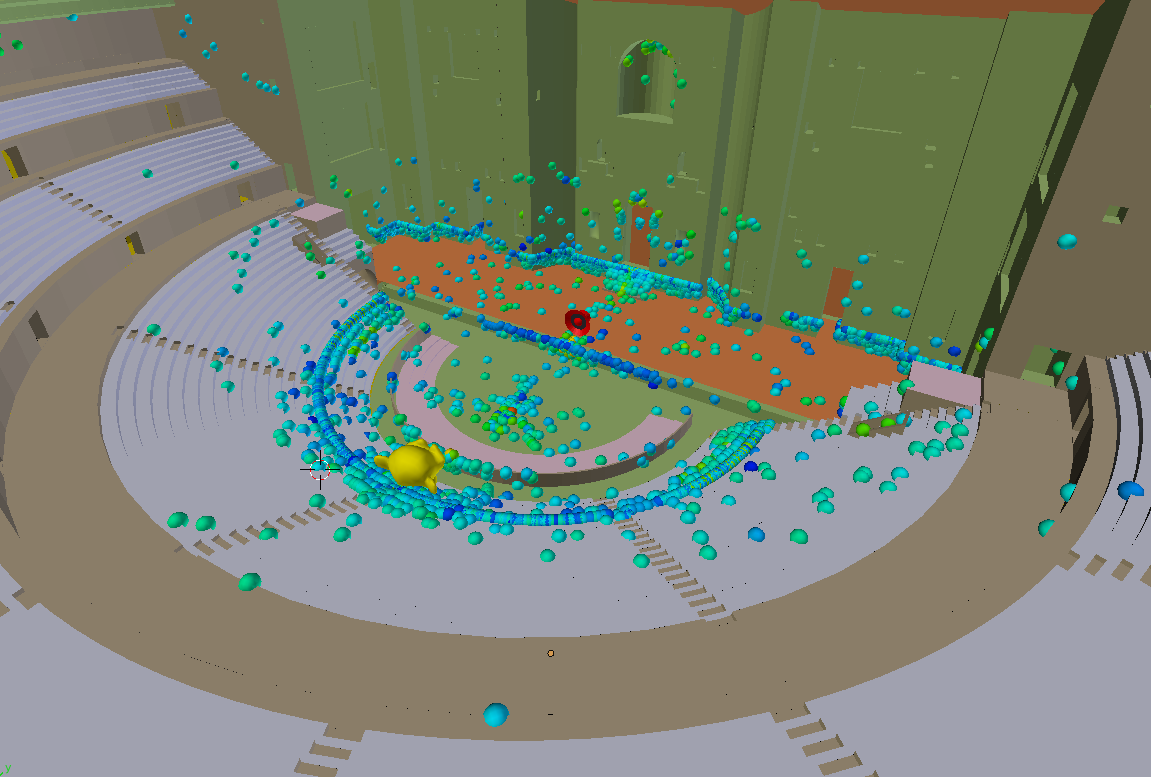
\includegraphics[width=\linewidth]{images/SIsansDec}
	\caption{Source-images projetées sur les parois du théâtre jusqu'à -60dB sans la décoration du front de scène.}
	\label{SIsansDec}
\end{figureth}

\begin{tableth} 
 \begin{tabular}{| *{9}{c|}} 
 \hline 
 Facteur & 62,5Hz & 125Hz & 250Hz & 500Hz & 1kHz & 2kHz & 4kHz & 8kHz \\ 
 \hline 
 \hline 
\gls{EDT} (ms)& 1436& 1387& 1211& 884& 709& 645& 594& 361 \\ 
 \hline 
\gls{T30} (ms)& 3886& 3827& 3049& 2745& 2477& 1969& 1315& 592 \\ 
 \hline 
\gls{G} (dB)& 5.8& 5.8& 5.4& 5& 4.8& 4.6& 4.1& 3.4 \\ 
 \hline 
\gls{C80} (dB)& 4.01& 4.04& 4.83& 5.41& 5.89& 6.68& 8.51& 13.37 \\ 
 \hline 
\gls{D50} (\%)& 61.01& 61.17& 63.81& 65.42& 67.04& 69.84& 76.22& 88.34 \\ 
 \hline 
\gls{Ts} (ms)& 84& 83& 68& 60& 53& 44& 28& 12 \\ 
 \hline 
\end{tabular} 
 \caption{Facteurs perceptifs pour une source en [0 ; 5.6 ; 42.8] et un auditeur en [0 ; -16.5 ; 43.9] et 1~000~000 de rayons sans décoration du front de scène.} 
 \label{tab_fact_sansdec} 
 \end{tableth}


\section{Position des spectateurs}
Le test suivant consiste à comprendre l'impact de la position dans les gradins. Nous savons que le placement dans la \gls{cavea} se faisait selon le rang social des spectateurs. Nous comprenons facilement que visuellement, les spectateurs les plus proches étaient ceux qui voyait le mieux les acteurs, même si ceux situés légèrement en recul avaient une meilleure vu d'ensemble. Ainsi nous avions les sénateurs sur des sièges mobiles dans l'orchestre, les chevaliers sur les premiers gradins puis la plèbe et pour finir les esclaves. Les tribunes étaient également occupées par des personnages importants.

Nous testons donc 12 nouvelles positions d'auditeur afin de comparer le signal perçu avec la \gls{rir} de référence (voir fig. \ref{position_rece}). Nous positionnons des séries d'auditeurs sur des axes à 0°, 55° et à 90° par rapport à la perpendiculaire au mur de scène. Sur chacun de ces axes, on positionne des récepteurs sur les derniers gradins des chaque \gls{maenianum} et pour les axes n'étant pas au niveau de l'\gls{aditus} on ajoute également des récepteurs au niveau des premiers gradins et de ceux de l'orchestre. On notera que les récepteurs 1, 5, 6 et 10 sont situés à l'emplacement de personnalités importantes.
\begin{figureth}
	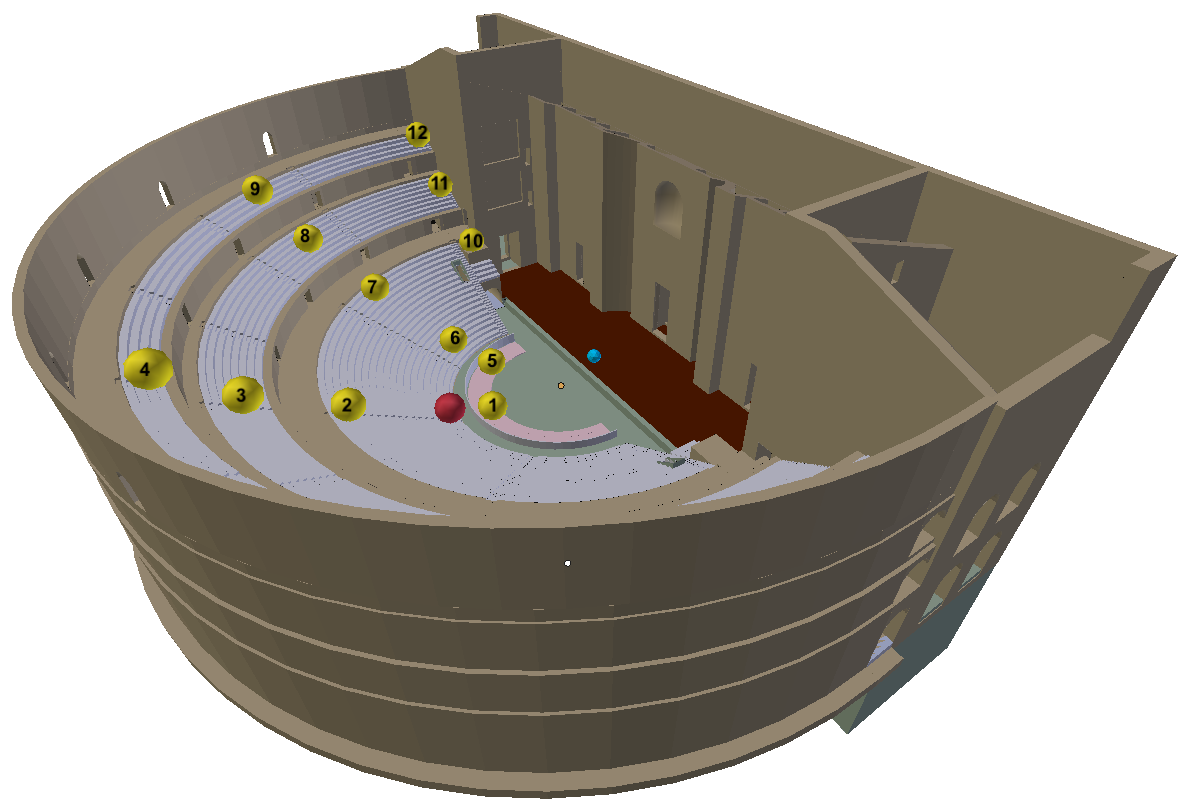
\includegraphics[width=\linewidth]{images/position_rece}
	\caption{Douze positions d'auditeurs (rose) à comparer à la position initiale (jaune).}
	\label{position_rece}
\end{figureth}
%
\begin{tableth} 
\footnotesize
 \begin{tabular}{| *{9}{c|}} 
 \hline 
 Récepteur & [x ; y ; z] (m)  & \gls{EDT} (ms) & \gls{T30} (ms) & \gls{spl} (dB) & \gls{C80} (dB) & \gls{D50} (\%) & \gls{Ts} (ms) \\ %& \gls{LF80} (dB) \\ 
 \hline 
 \hline 
1  & [0 ; -10.67 ; 41.44] &1310  &2861   &-29  &2.98  &60.14  &81 \\%listener12
 \hline 
 Réf    &[0 ; -16.5 ; 43.9] &1501  &2966   &-32  &3.65  &58.48  &81 \\%listenerREF
 \hline 
 2  & [0 ; -28.23 ; 50.02] &2163  &3690   &-35  &1.11  &42.03  &129 \\ %listener11
 \hline 
 3  &  [0 ; -37.86 ; 55.92] &2023  &4285   &-37  &0.31  &37.48  &133 \\ %listener10
 \hline 
 4  &  [0 ; -44.36 ; 62.06] &2439  &4335   &-37  &-0.72  &34.69  &155 \\%listener9
 \hline 
 \hline
 5  &   [-8.74 ; -6.12 ; 41.44] &1539  &2788   &-28  &3.81  &62.14  &80 \\%listener5
 \hline 
 6  &  [-13.51 ; -9.46 ; 43.86] &1479  &3383   &-31  &4.78  &64.28  &79 \\%listener4
  \hline 
  7 &   [-23.12 ; -16.19 ; 50.02] &2130  &3892   &-34  &3.22  &52.99  &119 \\ %listener6
 \hline 
 8  &  [-31.02 ; -21.72 ; 55.92] &2342  &3916   &-37  &1.89  &52.76  &140 \\ %listener7
 \hline 
 9  & [-36.34 ; -25.44 ; 62.06] &2893  &4444   &-38  &0.17  &38.92  &177 \\ %listener8
 \hline 
 \hline
 10  &  [-28.23 ; 1.66 ; 50.02] &2650  &4507   &-33  &-0.32  &39.73  &168 \\ %listener3
 \hline 
11   & [-37.87 ; 1.66 ; 55.92] &3189  & 3951  &-37  & -1.24 &41.56  &205 \\%listener2
 \hline 
12   & [-44.36 ; 1.66 ; 62.06] &3611  & 4487  & -36 &-2.66  &31.9  & 256\\ %listener1
 \hline 
\end{tabular} 
 \caption{Facteurs perceptifs pour différents récepteurs sur la bande de fréquence de 500Hz pour 1~000~000 de rayons.} 
 \label{tab_fac_rec} 
 \end{tableth}
 
 
On constate d'après le tableau \ref{tab_fac_rec} plusieurs choses. Tout d'abord, le niveau acoustique \gls{spl} diminue de 3dB entre les gradins mobiles de l'orchestre réservés aux sénateurs et les premiers gradins accessibles aux classes moins élevés tels que les chevaliers. Le son est donc entendu deux fois moins fort. La perte est de 10dB au sommet de la cavea ce qui implique que les classes les plus modestes entendaient le son de la scène dix fois moins fort que les sénateurs de l'orchestre. En ce qui concerne la compréhensibilité, on distinguera les récepteurs situés au dessus de l'\gls{aditus} des autres. Ainsi on constate d'après les facteurs de clarté (\gls{C80}) et de définition (\gls{D50}) que pour les récepteurs 10 à 11 la compréhensibilité est nettement dégradée. On comprend grâce à la figure \ref{listener11} que cela est dû principalement aux deux \glspl{basilique}. Celle située à l'est génère un fort écho éloigné du son direct de la largeur de la scène (alors que pour les récepteurs dans l'axe, l'écho généré par le mur de scène n'est séparé que par la profondeur de la scène). On a aussi une forte concentration de sources-images au niveau de la \gls{precinction} à l'est du théâtre. La basilique occidentale va quant à elle stocker le son plus longtemps comme une sorte d'entonnoir puisque l'auditeur est dans son angle. Nous pouvons également noter que la première réflexion qui se fait sur l'orchestre lorsqu'on est dans la \gls{cavea} se fait sur la scène lorsqu'on est au dessus des \glspl{aditus}. L'effet miroir est donc légèrement estompé. Au niveau de la tribune et donc du récepteur 10 (voir fig. \ref{listener10}) l'effet est différent puisque le son provient principalement de la partie occidentale du front de scène et l'arrière de la tribune de qui doit être particulèrement bien adapté pour l'écoute musicale.
On analyse par ailleurs que quel que soit l'axe, lorsqu'on s'éloigne de la scène le temps de réverbération augmente. Cela est dû au fait que les divers réflexions entre le mur de scène et l'arrière de l'auditeur sont plus longues lorsqu'on s'éloigne du mur. Les autres facteurs permettent de comprendre que la compréhensibilité se dégrade aussi avec l'éloignement. 
%
\begin{figureth}
	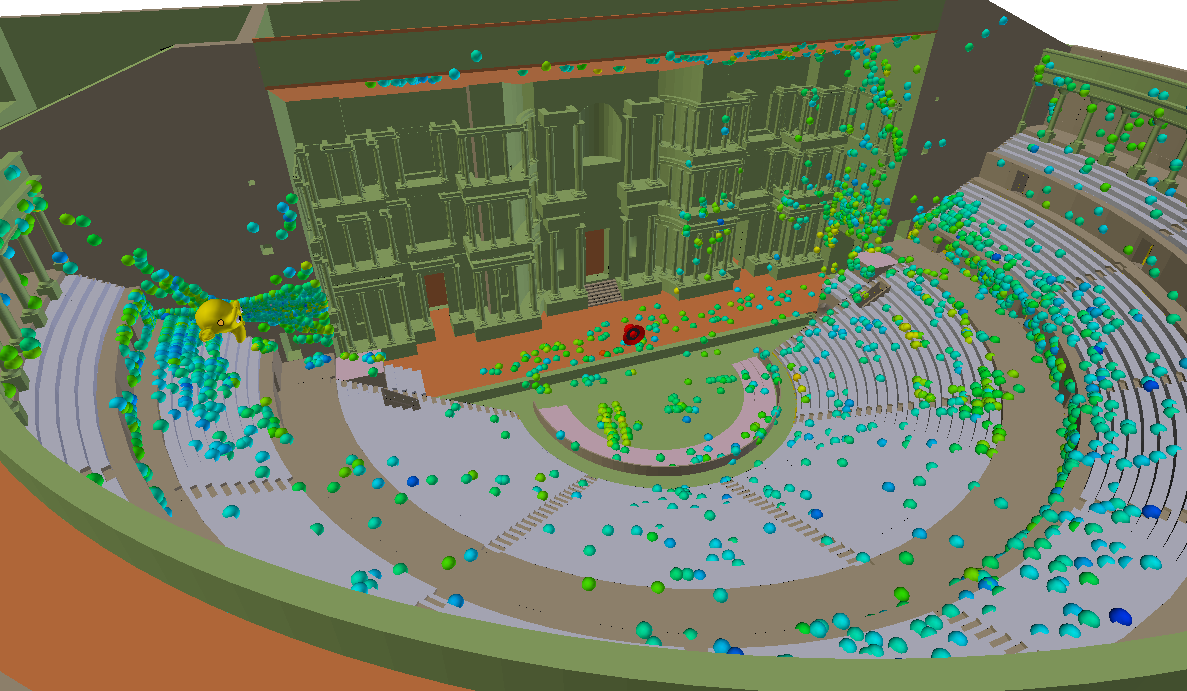
\includegraphics[width=\linewidth]{images/Listener11}
	\caption{Projection des sources-images pour un auditeur situé sur la tribune occidentale pour 1~000~000 de rayons.}
	\label{listener10}
\end{figureth}
\begin{figureth}
	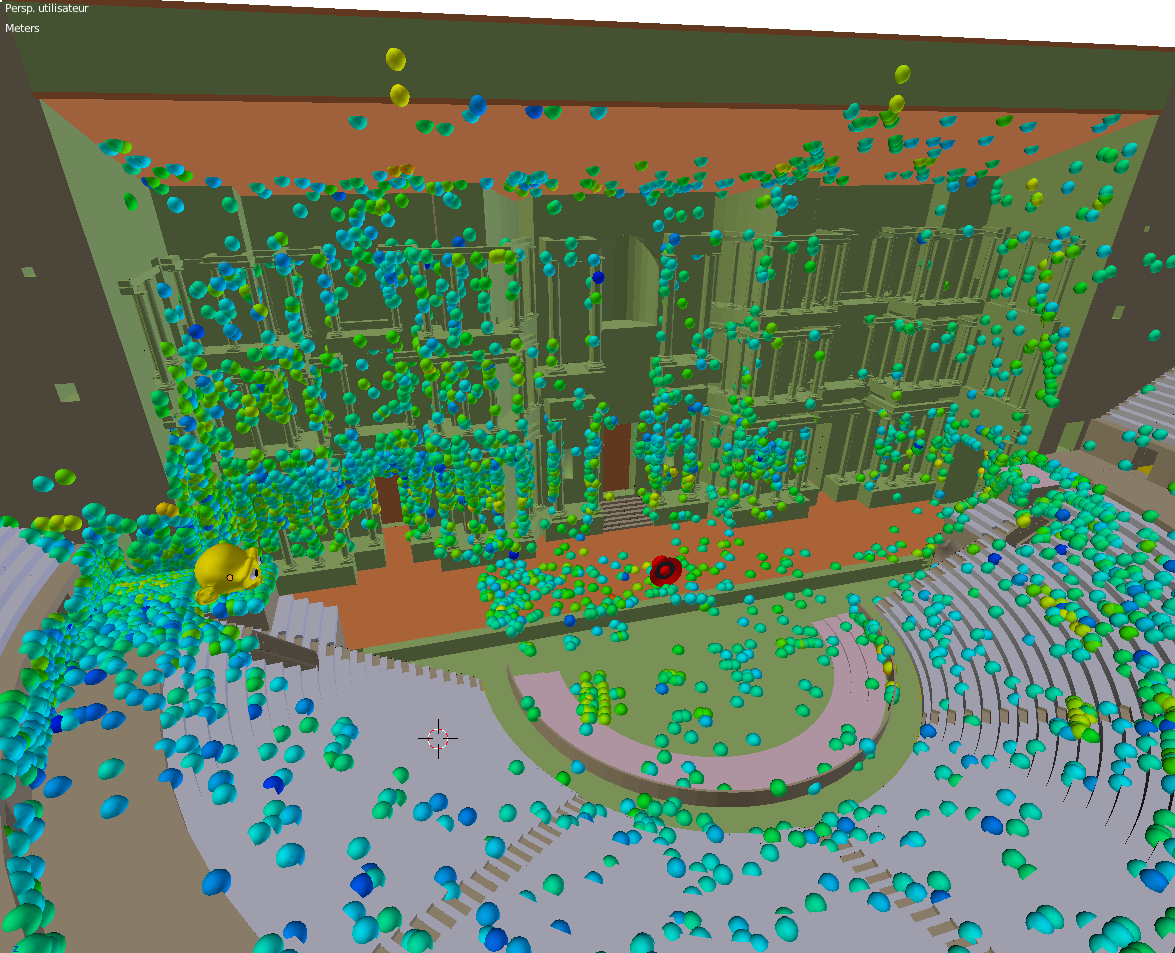
\includegraphics[width=\linewidth]{images/Listener10}
	\caption{Projection des sources-images pour un auditeur situé sur le deuxième \gls{maenianum} au dessus de l'\gls{aditus} occidental pour 1~000~000 de rayons.}
	\label{listener10}
\end{figureth}
%
%\begin{itemize}
%\item Pour l'axe perpendiculaire au mur de scène (récepteurs 1 à 4), la clarté (\gls{C80}) et la définition (\gls{D50}) restent bien adaptées à la transmission de la parole. Le temps de réverbération double entre les premiers et derniers gradins ce qui dégrade légèrement ces paramètres. Néanmoins, le temps central (\gls{Ts}) restant inférieur à 50ms, on conserve un phénomène d'échos faible.
%\item Le long de l'axe décalé de 55° (récepteurs 5 à 9), le temps central (\gls{Ts}) se décale beaucoup plus loin (jusqu'à 136ms pour les derniers gradins) ce qui implique une moins bonne compréhensibilité. Effectivement lorsque l'auditeur n'est pas bien dans l'axe, le signal se réfléchi sur les cotés de la \gls{cavea} (notamment sur les murs lisses tels que les \glspl{podium}) ce qui ajoute beaucoup de signal au champs diffus.  
%\item Dans le troisième axe (récepteurs 10 à 12) cet effet est encore amplifié puisque le son se réfléchi sur les \glspl{basilique}. Le temps de réverbération est plus important au niveau de la tribune car cet auditeur bénéficie de nombreuses réflexions sur le mur de scène que les auditeurs du deuxième et troisième \gls{maenianum} n'ont pas. On constate alors que sur cet axe, l'acoustique n'est plus vraiment adaptée à la parole mais plutôt à la musique.
%\end{itemize}
%Le paramètre \gls{LF80} (dB) n'apparait pas dans le tableau \ref{tab_fac_rec} car la valeur reste toujours très faible (<0,1dB) conséquence du fait que le son provenant de la scène est grandement majoritaire.

Pour résumer, les spectateurs les plus éloignés entendait le son jusqu'à dix fois moins fort. Plus on se rapproche de la scène, plus l'acoustique est favorable à la parole tandis que lorsqu'on s'approche de l'axe des \glspl{aditus} l'acoustique est plus favorable à la musique.

\section{La source et le mur de scène}

Au théâtre d'Orange il est probable que les sources sonores étaient composés d' ... (à completer)
ainsi leur directionnalité semble plutôt orientée vers le public et non vers le mur de scène. La fonction du mur semble donc dans un premier temps être décorative et isolante. Effectivement la structure complètement enclavante du théâtre coupe les spectateurs des bruits extérieurs. Par ailleurs la décoration détaillée du front de scène apporte inévitablement un effet de diffusion des  fréquences audibles. Néanmoins, on peut explorer l'impact de la forme caractéristique du mur de scène sur la réflexion du son. Cette dernière est liée est la position de la source sonore. La figure \ref{test_source1} montre les rayons se propageant vers le mur de scène et revenant vers les spectateurs (dans le plan à 1m60 au dessus de la scène) dans la configuration de référence sans décor. On constate que le mur autour de la porte centrale renvoi des rayons dans les gradins tandis que l'\gls{exedre} curviligne ainsi que les baldaquins en saillie renvoient les rayons vers les tribunes. La figure \ref{test_source2} représente le même test pour une source située sur l'axe entre les portes latérales menant aux \glspl{parascaenium} c'est-à-dire à Y=9m. On constate dans ce cas que l'\gls{exedre} curviligne permet de concentrer une partie des rayons sur les extrémités de la \gls{cavea}. De la même manière, grâce aux figures \ref{test_source3} et \ref{test_source4}, on constate bien que plus on s'éloigne du bord de la scène, plus l'\gls{exedre} concentre les rayons vers l'axe central de la \gls{cavea}. On voit d'ailleurs sur la figure \ref{test_source4} que lorsque la source est sur l'escalier de la porte royale, (quasiment dans l'encadrement), les rayons reviennent de part et d'autre de l'escalier central de la \gls{cavea}. 

\begin{figureth}
	\begin{subfigureth}{0.48\textwidth}
		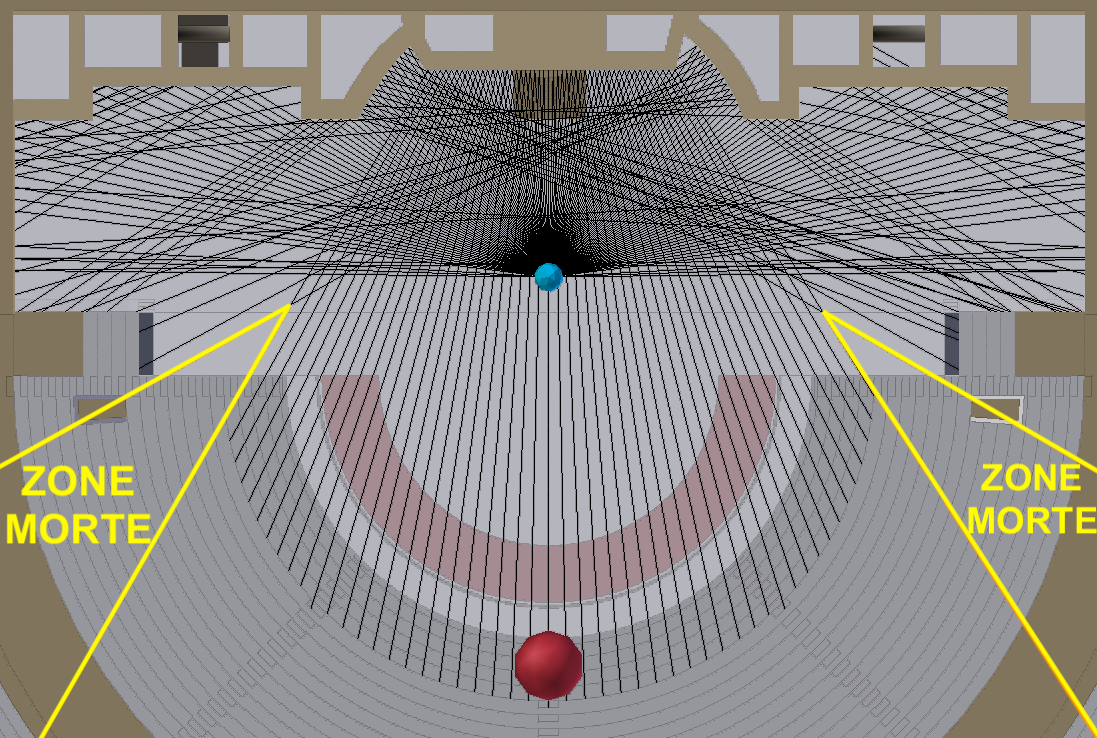
\includegraphics[width=\linewidth]{images/test_source1}
		\caption{Reflexion des rayons sur le mur de scène pour une source située en [0 ; 3,6 ; 42,8].}
		\label{test_source1}
		\hfill
		\quad
	\end{subfigureth}
	\quad
	\begin{subfigureth}{0.48\textwidth}
		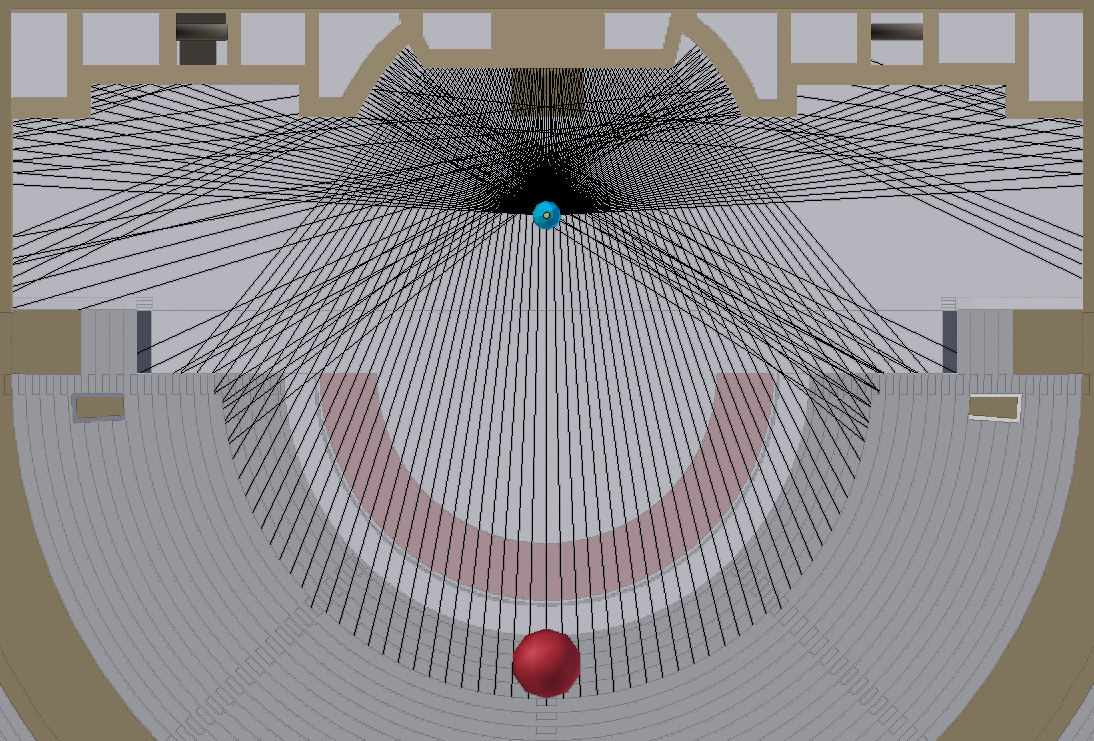
\includegraphics[width=\linewidth]{images/test_source2}
		\caption{Reflexion des rayons sur le mur de scène pour une source située en [0 ; 9 ; 42,8].}
		\label{test_source2}
		\quad
	\end{subfigureth} 
	\begin{subfigureth}{0.48\textwidth}
		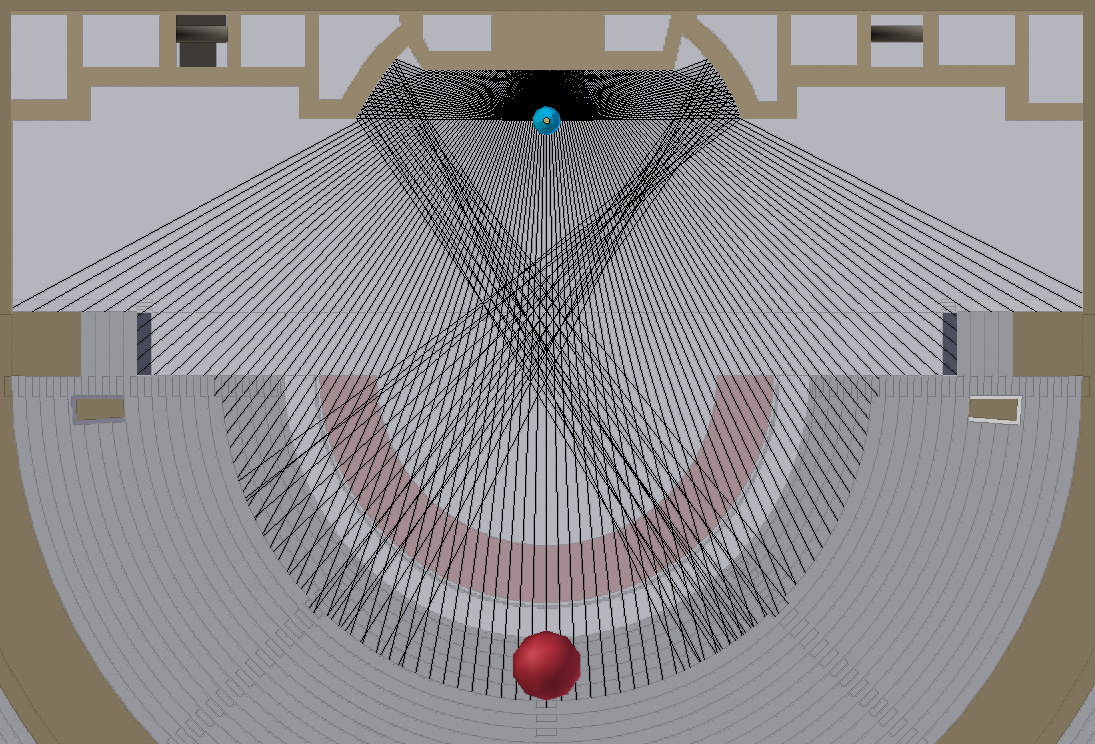
\includegraphics[width=\linewidth]{images/test_source3}
		\caption{Reflexion des rayons sur le mur de scène pour une source située en [0 ; 14,5 ; 42,8].}
		\label{test_source3}
	\end{subfigureth}
	\quad
	\begin{subfigureth}{0.48\textwidth}
		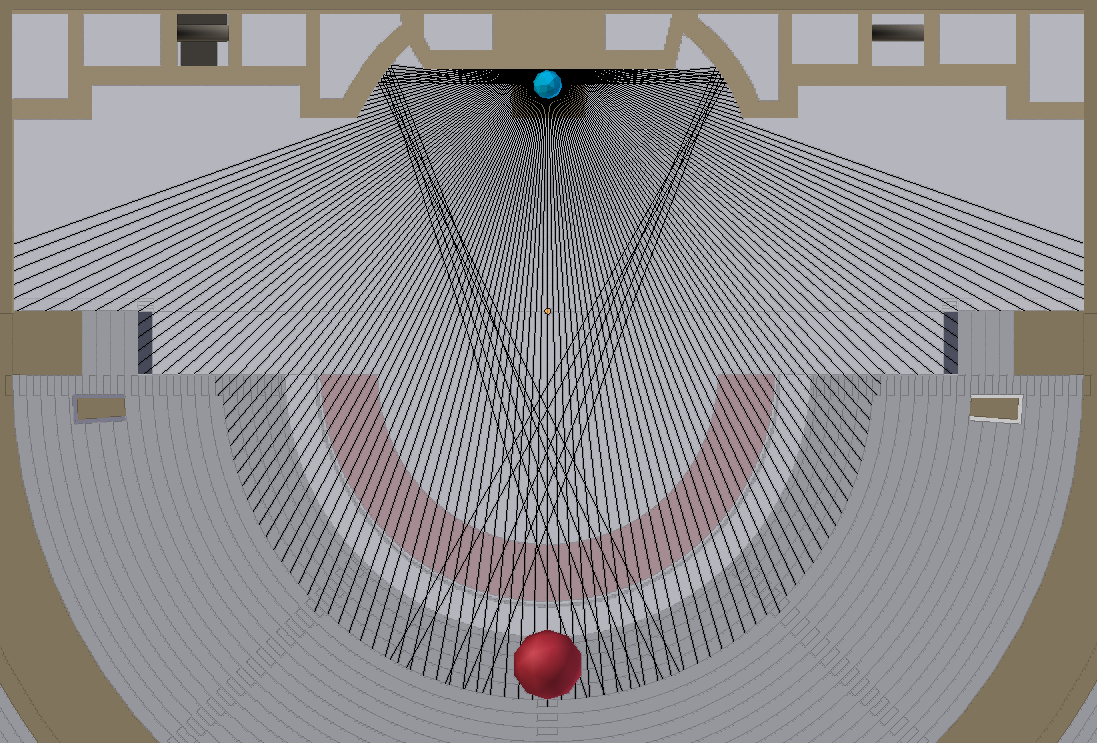
\includegraphics[width=\linewidth]{images/test_source4}
		\caption{Reflexion des rayons sur le mur de scène pour une source située en [0 ; 16,5 ; 42,8].}
		\label{test_source4}
	\end{subfigureth}
\caption{Reflexion des rayons propagés depuis une source vers le mur de scène dans un plan horizontal.}	
\label{test_source}
\end{figureth}	

Si on se place maintenant dans le plan vertical YZ (ou vu de profil). Nous avons vu précédemment que la reflexion sur l'orchestre est très importante puisqu'elle permet de renvoyer une grande partie des rayons vers les gradins. Cependant, plus la source va s'éloigner du bord de la scène moins il y aura de rayons réfléchis sur l'orchestre. Les rayons sont alors réfléchis sur la scène qui possèdes des coefficients d'absorption plus élevés. On peut alors calculer la distance $d$ de l'orchestre qui va réfléchir des rayons en fonction de la distance $d'$ de la source sur la scène par rapport au bord (voir fig \ref{angle_refl}). D'après le théorème de Thalés on a :
\begin{equation}
d = \frac{h'}{h}\times d' = 1,33d',
\end{equation}
où :
\begin{itemize}
\item h est la hauteur de la scène (1,2m à Orange),
\item h' est la hauteur de la source sur la scène (1,6 m en prenant en compte la taille moyenne d'un acteur).
\end{itemize}
Ainsi, lorsque que l'acteur s'éloignera du bord de la scène de 1m, les réflexions se feront sur 1,33m de moins sur l'orchestre. On note par ailleurs que les escaliers de la porte royales se trouvent à 11m du bord de la scène ; lorsque l'acteur sera à cette position, les rayons ne toucherons l'orchestre qu'à 14,63m du bord de la scène ce qui tombe en plein dans les gradins mobile. Un acteur se trouvant en fond de scène ne bénéficiera donc pas de la reflexions sur l'orchestre pour amplifier le son.
\begin{figureth}
	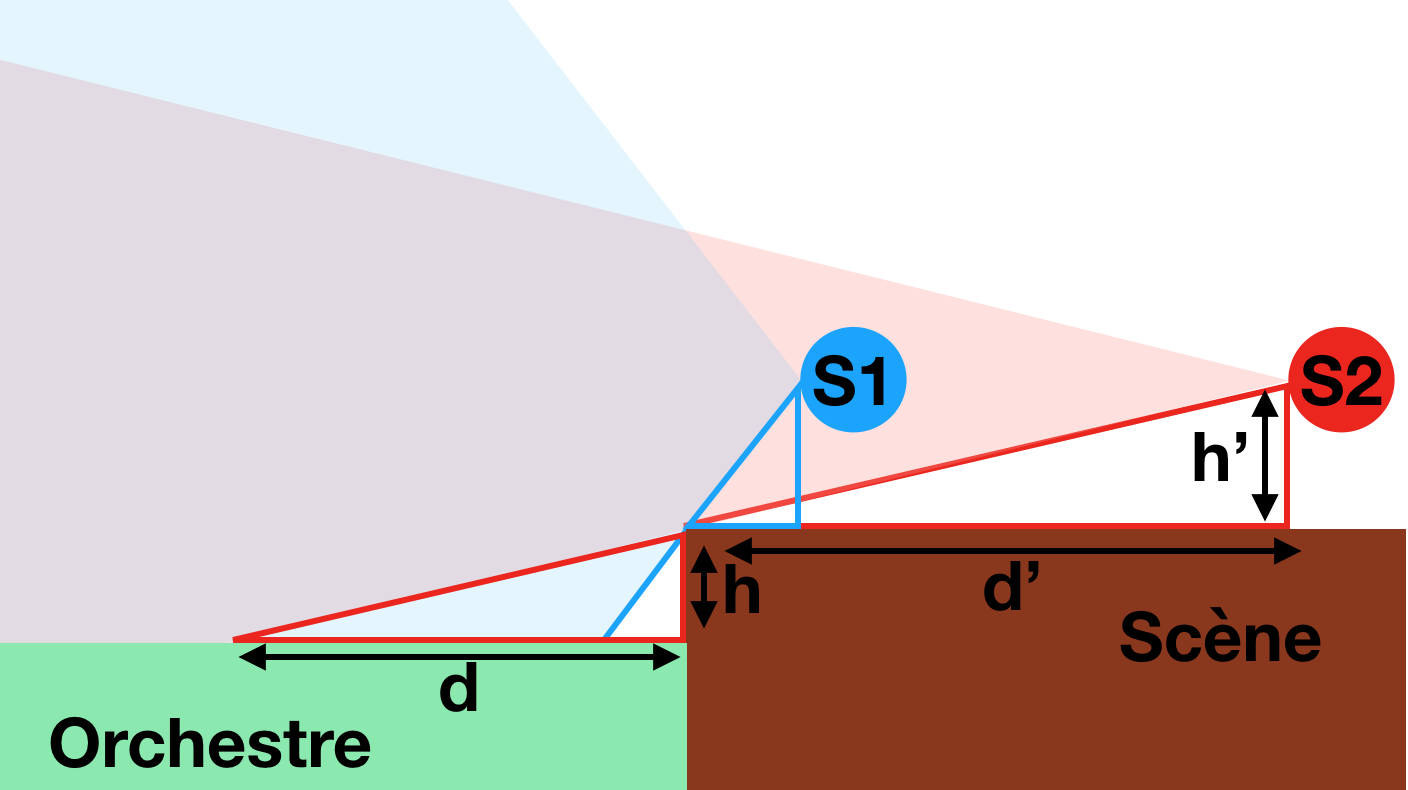
\includegraphics[width=0.8\linewidth]{images/angle_refl}
	\caption{Vu de profil de la propagation sonore à partir de deux sources S1 et S2. Proportion de signal réfléchi sur l'orchestre plus faible pour S2 que pour S1.}
	\label{angle_refl}
\end{figureth}

%\section{L e mur de scène}	

%on ajoute l'escalier central 

%qt mettre niveau en db pour le nom des source images rvb


\section{Absorption des spectateurs et du \gls{velum}}
\cite[p.212]{jouhaneau}
%\section{Présence de velum}
\section{Les couvertures de la scène et de la \gls{porticus isc}}
%\section{Impact du bruit extérieur}

\newpage

\chapter{Comparaison avec d'autres théâtres antiques}
\citationChap{
Si on veut connaitre un peuple, il faut écouter sa musique
}{Platon}
\minitoc
\newpage

Citer  \cite[p.25]{rindel}

\begin{figureth}
	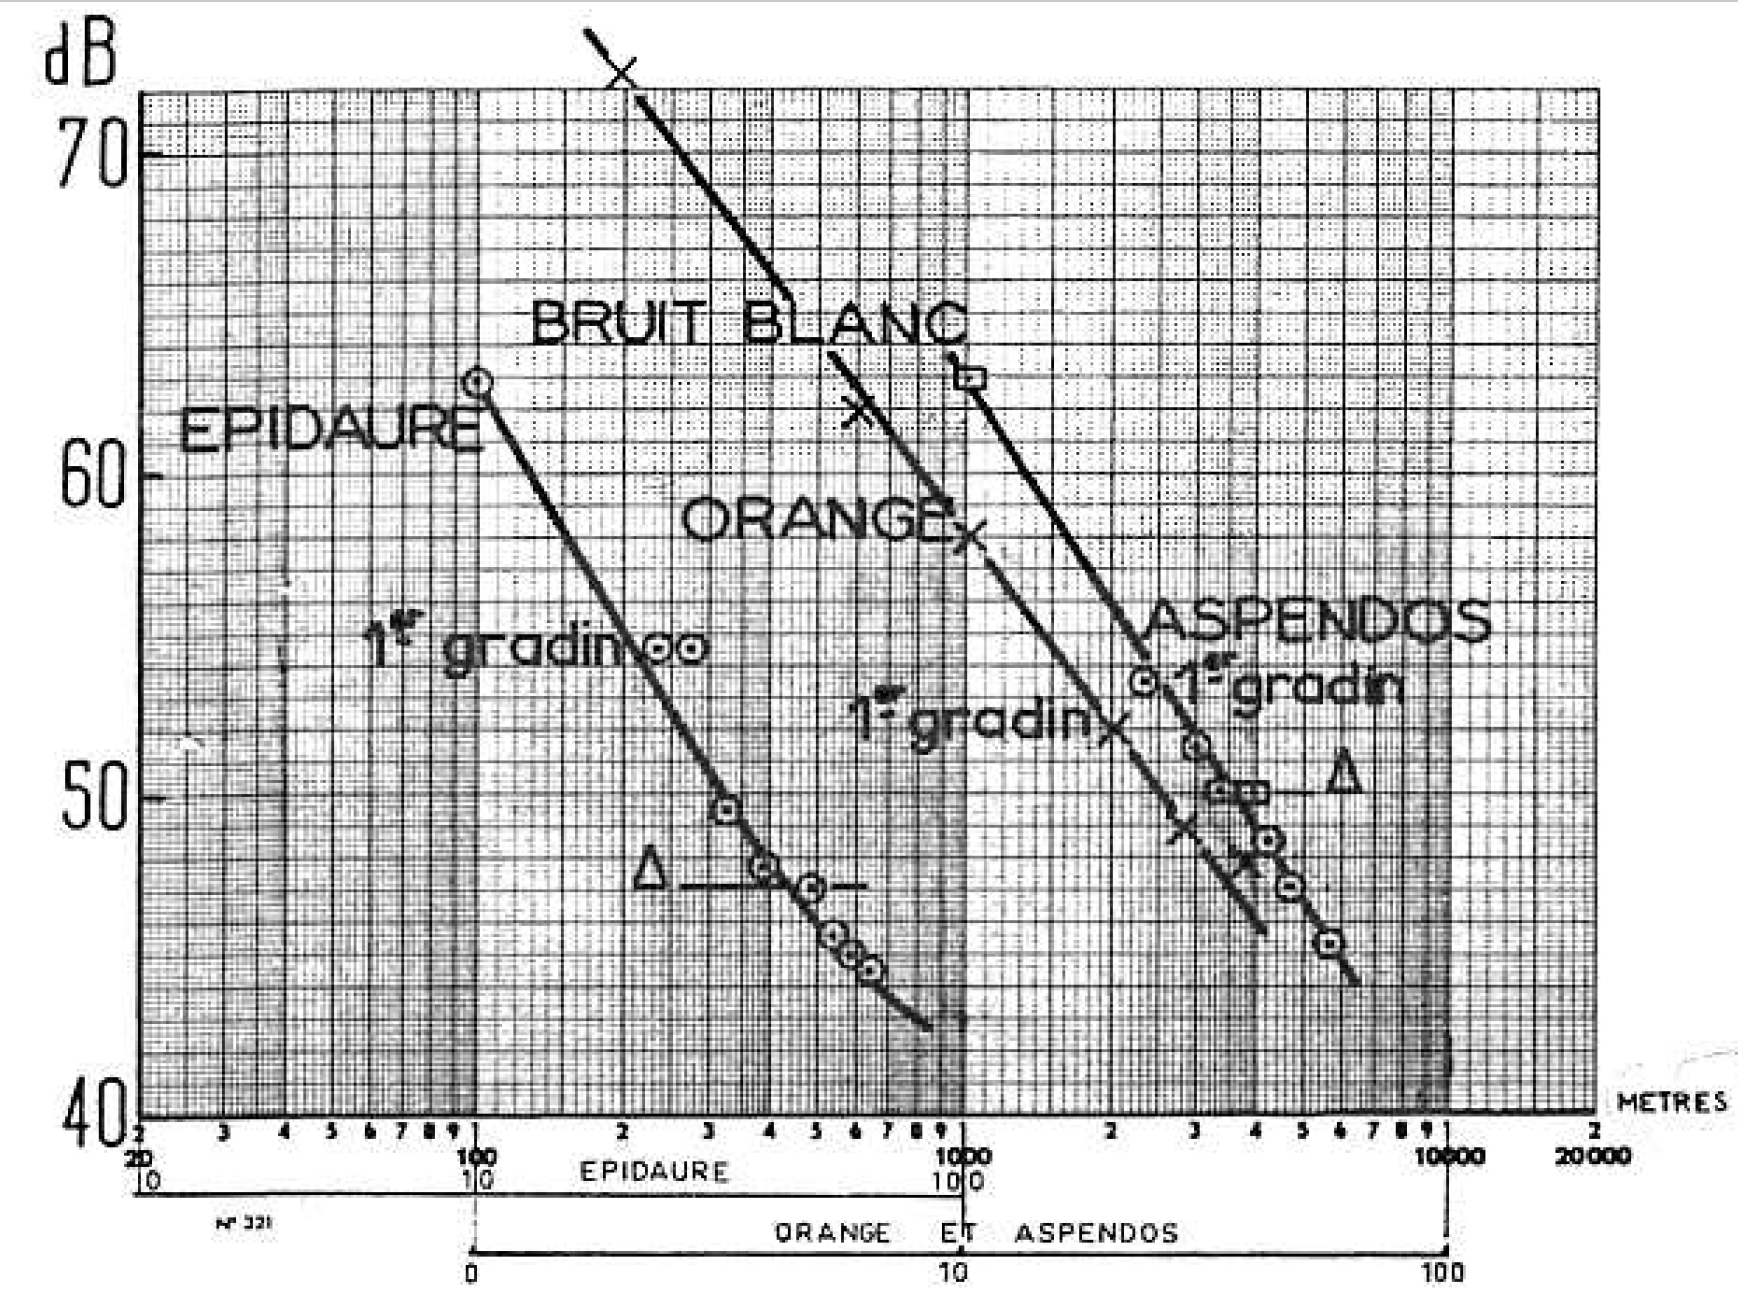
\includegraphics[width=0.7\linewidth]{images/canac_comparaison}
	\caption[Comparaison de l'intensité perçue entre les théâtre d'Epidaure, Aspendos et Orange.]{Comparaison de l'intensité perçue entre les théâtre d'Epidaure, Aspendos et Orange \footnotemark.}
	\label{canac_comparaison}
\end{figureth}
\citefnt[p.162]{canac}
%
\begin{figureth}
	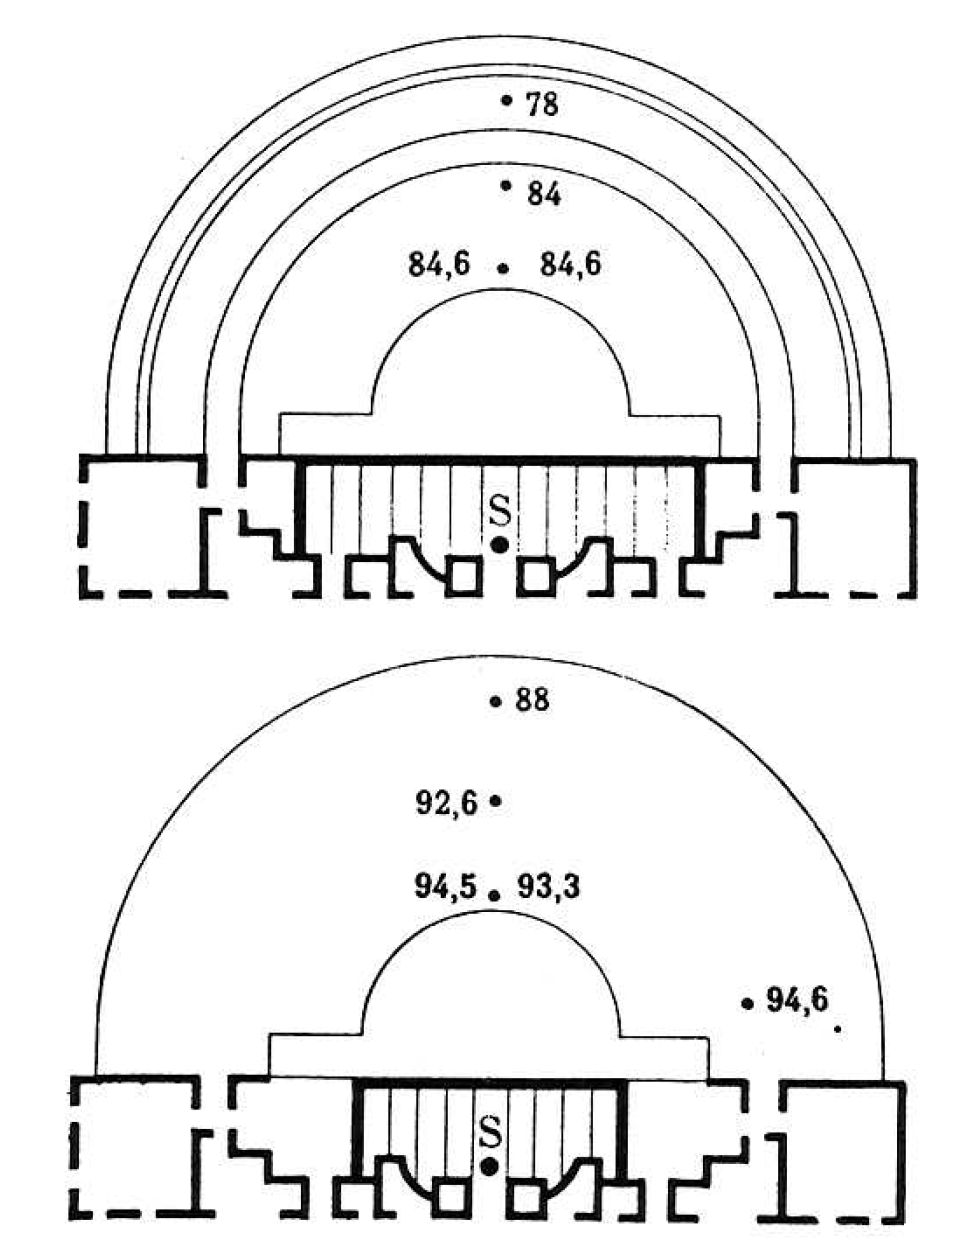
\includegraphics[width=0.7\linewidth]{images/canac_comparaison2}
	\caption[Comparaison de la compréhensibilité à Orange, avec un mur (en haut) et à Vaison, sans mur (en bas).]{Comparaison de la compréhensibilité à Orange, avec un mur (en haut) et à Vaison, sans mur (en bas) \footnotemark.}
	\label{canac_comparaison2}
\end{figureth}
\citefnt[p.152]{canac}

\begin{figureth}
	\begin{subfigureth}{0.48\textwidth}
		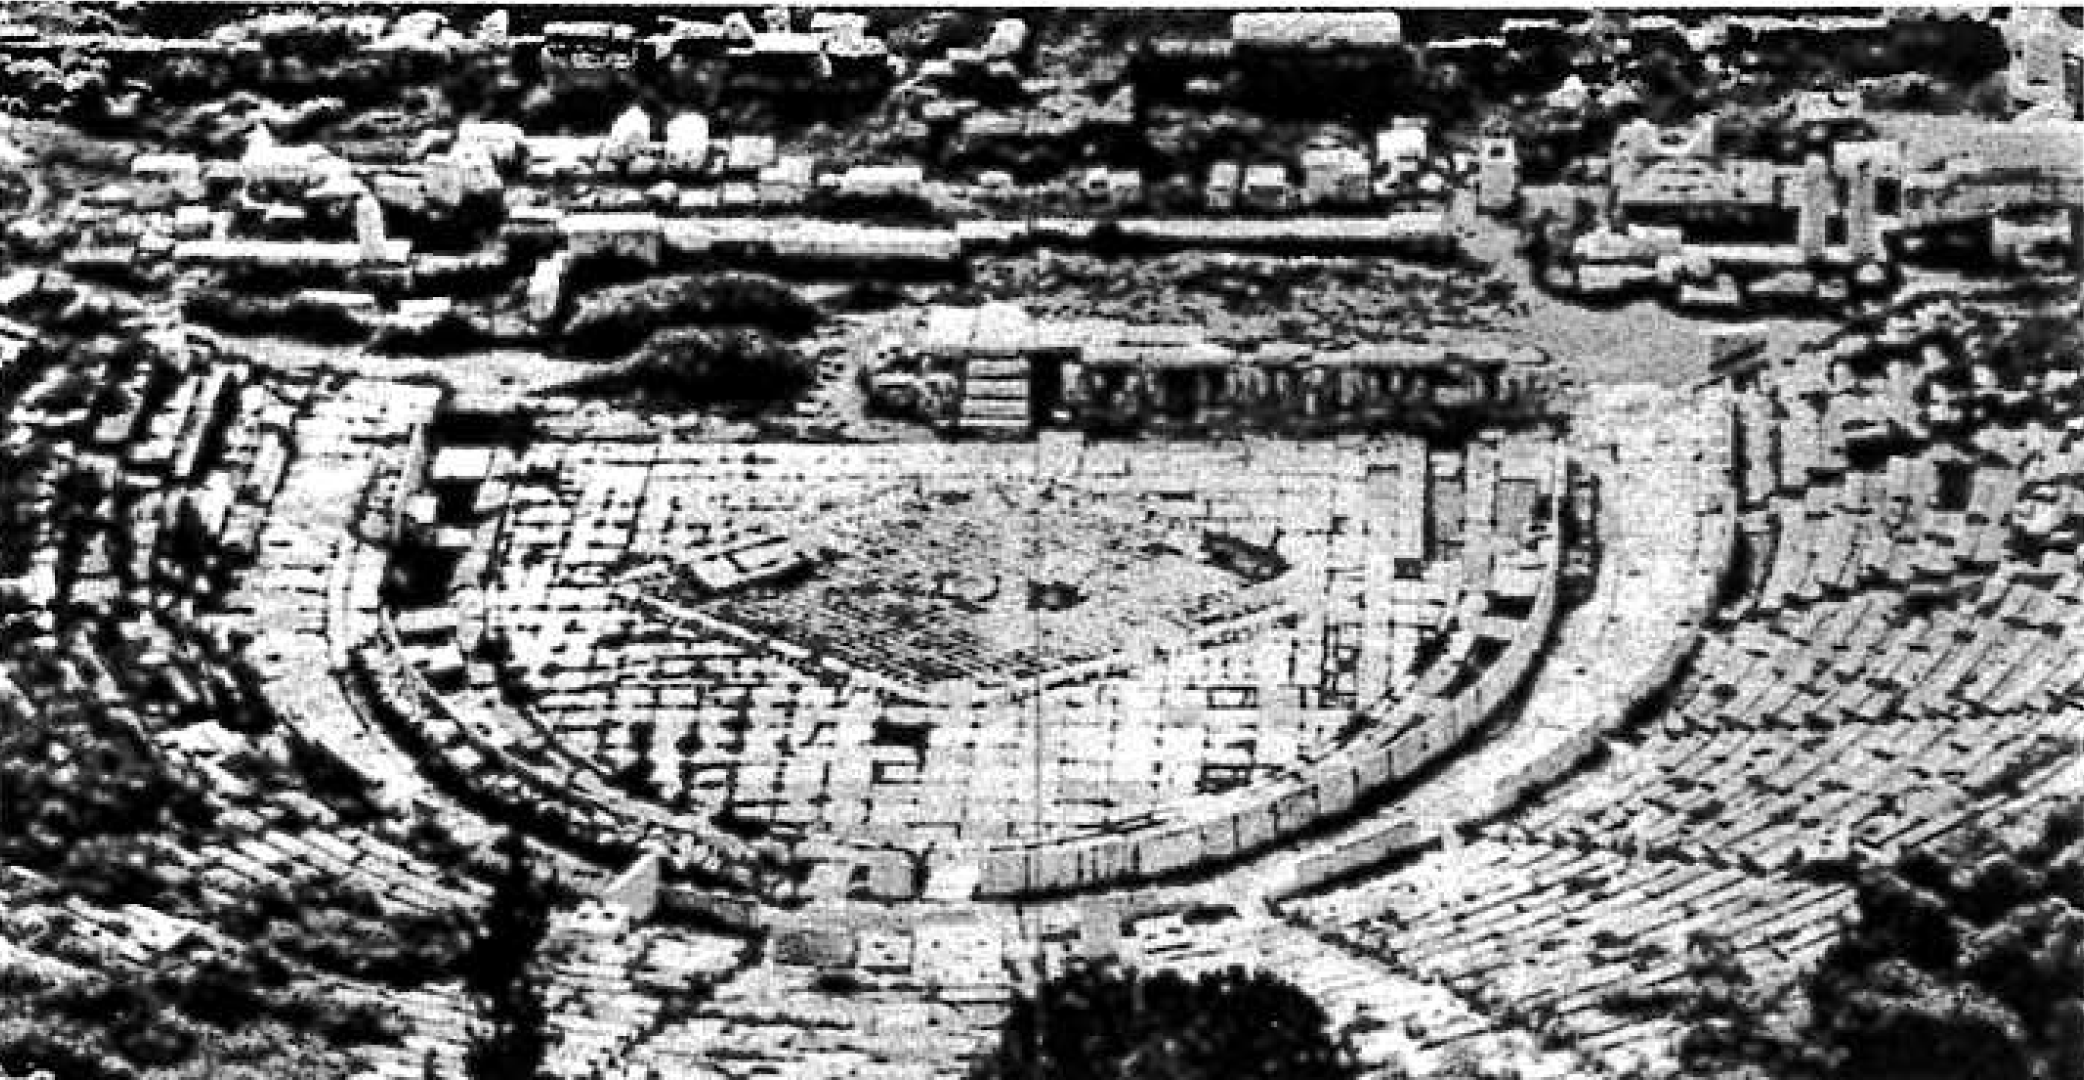
\includegraphics[width=\linewidth]{images/dyonisos1}
		\caption[Mosaïque en losange dans l'orchestre du théâtre de Dyonisos à Athènes.]{Mosaïque en losange dans l'orchestre du théâtre de Dyonisos à Athènes \footnotemark.}
		\label{dyonisos1}
		\hfill
		\quad
	\end{subfigureth}
	\quad
	\begin{subfigureth}{0.48\textwidth}
		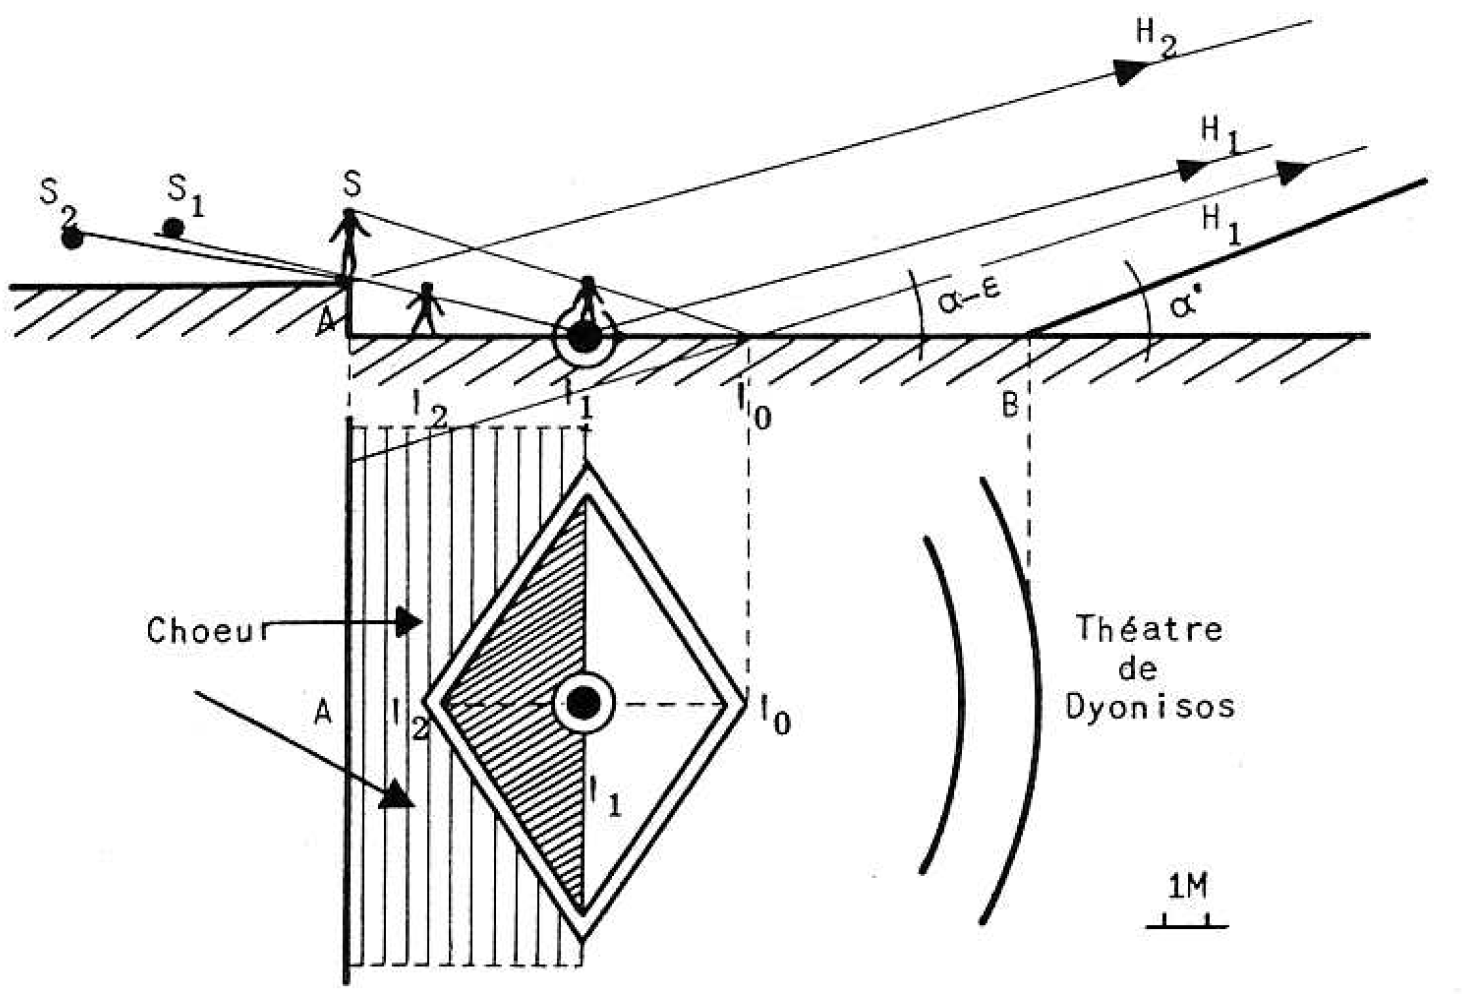
\includegraphics[width=\linewidth]{images/dyonisos2}
		\caption[Rôle supposé du losange dans l'orchestre du théâtre de Dyonisos. Emplacement du choeur.]{Rôle supposé du losange dans l'orchestre du théâtre de Dyonisos. Emplacement du choeur \footnotemark.}
		\label{dyonisos2}
		\quad
	\end{subfigureth} 
\caption{Analyse de l'orchestre du théâtre de Dyonisos à Athènes.}	
\label{dyonisos}
\end{figureth}	
\addtocounter{footnote}{-1}
\citefnt[Fig. V-7 bis - p.119]{canac}
\addtocounter{footnote}{1}
\citefnt[Fig. V-7 - p.118]{canac}

\chapter*{Conclusion}
\addcontentsline{toc}{chapter}{Conclusion}

\newpage

% Biblio
 \bibliographystyle{francaissc}
 \bibliography{Part3/Biblio}
\addcontentsline{toc}{chapter}{Références}
